\documentclass[openany]{book}

% Preamble

\usepackage[margin=1in]{geometry}
\usepackage{amsfonts, amsmath, amssymb}
\usepackage{fancyhdr, float, graphicx}
\usepackage[utf8]{inputenc} % Required for inputting international characters
\usepackage[T1]{fontenc} % Output font encoding for international characters
\usepackage{fouriernc} % Use the New Century Schoolbook font
\usepackage[nottoc, notlot, notlof]{tocbibind}
\usepackage{listings}
\usepackage{xcolor}
\usepackage{blindtext}
\usepackage{hyperref}
\hypersetup{
    colorlinks=true,
    linkcolor=black,
    filecolor=magenta,      
    urlcolor=black,
    pdfpagemode=FullScreen,
    }

\definecolor{codegreen}{rgb}{0,0.6,0}
\definecolor{codegray}{rgb}{0.5,0.5,0.5}
\definecolor{codepurple}{rgb}{0.58,0,0.82}
\definecolor{backcolour}{rgb}{0.95,0.95,0.92}

\lstdefinestyle{mystyle}{
    backgroundcolor=\color{backcolour},   
    commentstyle=\color{codegreen},
    keywordstyle=\color{magenta},
    numberstyle=\tiny\color{codegray},
    stringstyle=\color{codepurple},
    basicstyle=\ttfamily\footnotesize,
    breakatwhitespace=false,         
    breaklines=true,                 
    captionpos=b,                    
    keepspaces=true,                 
    numbers=left,                    
    numbersep=5pt,                  
    showspaces=false,                
    showstringspaces=false,
    showtabs=false,                  
    tabsize=2
}

\lstset{style=mystyle}

% Header and Footer
\pagestyle{fancy}
\fancyhead{}
\fancyfoot{}
\fancyhead[L]{\textit{{Information and Cybersecurity}}}
\fancyhead[R]{\textit{\small{Krishnaraj T}}}
%\fancyhead[R]{\textit{something}}
\fancyfoot[C]{\thepage}
\renewcommand{\footrulewidth}{1pt}



% Other Doc Editing
% \parindent 0ex
%\renewcommand{\baselinestretch}{1.5}



% \title{Your Book Title}
% \author{Your Name}
% \date{\today}

\begin{document}

\begin{titlepage}
	\centering

	%---------------------------NAMES-------------------------------


	
\includegraphics[width=0.7\textwidth]{Final-MIT-WPU-logo-page-001.jpg}\par\vspace{1cm}
	\huge\textsc{
		School of Computer Engineering and Technology
	}\\

	\vspace{0.75\baselineskip} % space after Uni Name

	\LARGE{
		Cybersecurity and Forensics
	}

	\vfill % space after Sub Name

	%--------------------------TITLE-------------------------------

	\rule{\textwidth}{1.6pt}\vspace*{-\baselineskip}\vspace*{2pt}
	\rule{\textwidth}{0.6pt}
	\vspace{0.75\baselineskip} % Whitespace above the title



	\huge{\textsc{
			Information and Cybersecurity\\
			CET3004B
		}} \\



	\vspace{0.5\baselineskip} % Whitespace below the title
	\rule{\textwidth}{0.6pt}\vspace*{-\baselineskip}\vspace*{2.8pt}
	\rule{\textwidth}{1.6pt}

	\vspace{1\baselineskip} % Whitespace after the title block

	%--------------------------SUBTITLE --------------------------	

	\LARGE\textsc{
		Subject Manual
	} % Subtitle or further description
	\vfill

	%--------------------------AUTHOR-------------------------------

	Prepared By
	\vspace{0.5\baselineskip} % Whitespace before the editors

	\Large{
		Prof. Umesh Raut \\
	}


	\vspace{0.5\baselineskip} % Whitespace below the editor list
	% \today

\end{titlepage}


\tableofcontents
\frontmatter
% \maketitle

\chapter{Course Objectives}
\section{Knowledge}
\begin{enumerate}
	\item  To focus on the models, tools, and techniques for enforcement of security with some emphasis on
	      the use of cryptography. Students will learn security from multiple perspectives
	\item To educate students on the fundamental principles and techniques of computer and network
	      security1
\end{enumerate}

\section{Skills}
\begin{enumerate}
	\item Acquire background on hash functions, authentication, firewalls, intrusion detection techniques
	\item Gain hands-on experience with programming and simulation techniques for security protocols
\end{enumerate}


\section{Attitude}
\begin{enumerate}
	\item Understand the tradeoffs and criteria/concerns for security countermeasure development
	\item Learn to apply methods for authentication, access control, intrusion detection and prevention
\end{enumerate}

\chapter{Course Outcomes}
\begin{enumerate}
	\item Analyze and resolve security issues in networks and computer systems to secure an IT
	      infrastructure.
	\item Apply methods for authentication, access control, intrusion detection and prevention.
	\item Develop policies and procedures to manage enterprise security risks.
	\item Evaluate and communicate the human role in security systems with an emphasis on ethics,
	      social engineering vulnerabilities and training.
	\item Identify software security vulnerabilities, summarize and mitigate security risks associated
	      with integrating systems.
\end{enumerate}

\chapter{Course Contents}
\section{Module 1}

\subsection{Foundations of Information Security}
Information Security fundamentals, it's need,
Confidentiality, Integrity, Availability (CIA triad), Security Policies, Procedures, Guidelines,
Standards Administrative Measures and Technical Measures, Attacks, Vulnerability, Security
Goals, Security Services and Defense mechanisms

\subsection{Cryptographic Techniques}
Conventional substitution and transposition ciphers, One-time Pad, Block cipher and Stream
Cipher, Cipher modes of operations, Steganography. Symmetric Cryptographic Techniques: DES,
AES\\

\noindent
\textbf{Time Required: 9 Hours}


\section{Module 2}

\subsection{Mathematical Foundations and Public Key Cryptography}
Mathematics for Security: Modular Arithmetic, Euler's theorem, Fermat Theorem, Euclidean
Algorithm, Miller-Rabin Algorithm, Primality Test, Chinese Remainder Theorem, Discrete
Logarithm, Asymmetric Key Cryptography: RSA algorithms. Hash algorithms: MD5, SHA1\\

\noindent
\textbf{Time Required: 9 Hours}


\section{Module 3}

\subsection{Foundations of Information Security}
Use of Cryptography for authentication, Secure Hash function, Key Management and Distribution:
Symmetric Key Distribution, Using Symmetric Encryption, Symmetric Key Distribution Using
Asymmetric Encryption, Distribution of Public Keys, Cryptographic Key Infrastructures, Diffie-Hellman Key Exchange, Digital Certificates x509.
Authentication Protocols: Remote, Mutual Authentication, Authentication Methods: Password,
Two way methods, Biometric Authentications, Kerberos Security\\



\noindent
\textbf{Time Required: 9 Hours}


\section{Module 4}

\subsection{Network and Cyber Security}
Networks Security Fundamentals, Layer-wise Security concerns, Firewalls: Packet filtering,
Stateless and Stateful, Intrusion detection systems: host based, network based IDS, Secured Socket
Layer Security, IP level IPSEC security, Email Security: PGP, S/MIME.
Cyber Security: Definition and origin, Cyber Crime and information security, Types of Cyber
Crime, Classification of Cyber Criminals, Tools used in Cyber Crime, Challenges, Strategies, The
Legal Perspective-Indian/Global Perspective, Types of Attack, Social Engineering, Cyber stalking,
Ransomware.\\


\noindent
\textbf{Time Required: 9 Hours}


\section{Module 5}

\subsection{Cybersecurity Techniques, Tools and Laws}
Introduction, Proxy servers and Anonymizers, Phishing, Password Cracking tools, Key-loggers
and Spywares, DoS and DDoS, Viruses, Worms, Trapdoors, Salami attack, Man-in-the- middle
attacks, Covert channels, SQL injection, Cyber Security Safeguards- Overview, Access control,Audit, Authentication, Biometrics. Cybercrime and Legal perspectives, Cyber laws Indian context,
The Indian IT Act-Challenges, Amendments, Challenges to Indian Law and cybercrime Scenario in
India, Indian IT Act and Digital Signatures.\\


\noindent
\textbf{Time Required: 9 Hours}

\chapter{References and Further Reading}
\section{Books}
\begin{enumerate}
	\item Michael E. Whitman and Herbert J. Mattord, “Principles of Information Security”, Cengage Learning;
	      ISBN: 1285448367
	\item Christof Paa and Jan Pelzl, “Understanding Cryptography: A Textbook for Students and Practitioners”,
	      Springer; ISBN: 3642041000
	\item William Stallings and Lawrie Brown, “Computer Security: Principles and Practice”, Prentice Hall.
	      Swiderski, Frank and Syndex, “Threat Modeling”, Microsoft Press.
	\item Ohn W. Rittinghouse, William M. Hancock, “Cyber Security Operations Handbook”, Elsevier Pub.
	\item Deborah G Johnson, “Computer Ethics”, 4th Edition, Pearson Education Publication.
	\item Earnest A. Kallman, J.P Grillo, “Ethical Decision making and IT: An Introduction with Cases”,
	      McGraw Hill Publication.
\end{enumerate}

\section{Other Resources}
\subsection{Web Resources}
\url{https://www.newhorizons.com/promotions/cybersecurity-ebooks}\\

\noindent
\subsection{MOOCs and Weblinks}
\noindent
COURSERA, NPTEL, etc.\\
\url{https://nptel.ac.in/courses/106106129}\\
\url{https://www.udemy.com/course/hands-on-penetration-testing-labs-30/}

\chapter{Guidelines for CCA and LCA}

\begin{figure}[H]
	\centering
	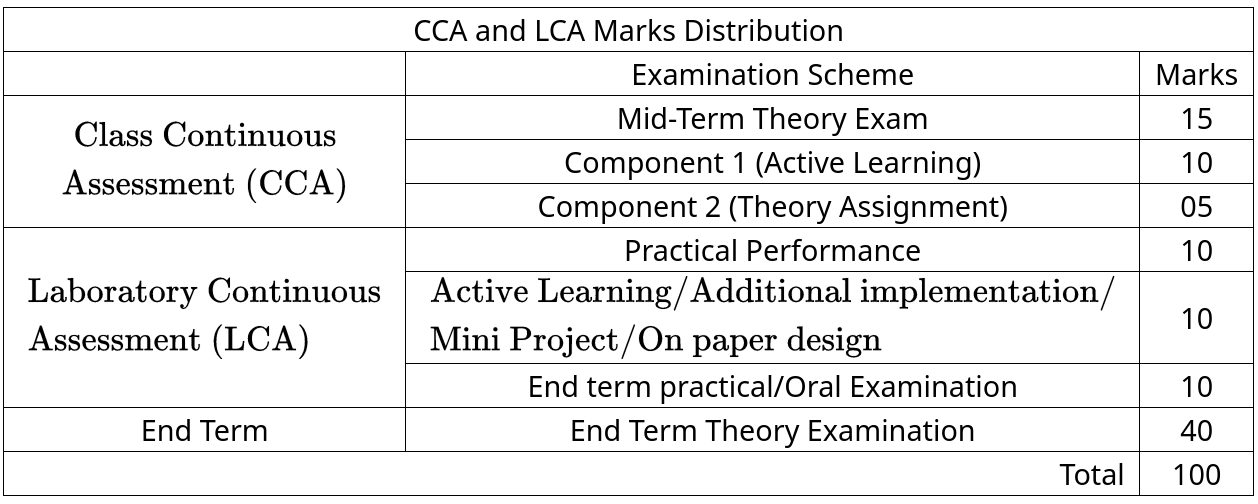
\includegraphics[width=.99\textwidth]{./cca.png}
\end{figure}
\mainmatter

\chapter{Classical Cryptographic Techniques}

\section{Aim}
Write a program using JAVA or Python or C++ to implement any classical cryptographic
technique.

\section{Objectives}
To conceal the context of some message from all accept the sender and recipient.

\section{Theory}

\subsection{Cryptography}

Cryptography is the practice and study of techniques for secure communication in the presence of third parties called adversaries. More generally, cryptography is about constructing and analyzing protocols that prevent third parties or the public from reading private messages; various aspects in information security such as data confidentiality, data integrity, authentication, and non-repudiation are central to modern cryptography. \\

\subsection{Types of Cryptography}

\subsubsection{Classical Cryptography}

Classical cryptography is the study of cryptography before the advent of modern computers. The classical ciphers are those ciphers that were in use before the advent of computers.

Some Classical Cryptographic Techniques are:

\begin{enumerate}
	\item \textit{Caesar Cipher} - A Caesar cipher is a type of substitution cipher in which each letter in the plaintext is replaced by a letter some fixed number of positions down the alphabet. For example, with a left shift of 3, D would be replaced by A, E would become B, and so on. The method is named after Julius Caesar, who used it in his private correspondence.

	      \begin{verbatim}
		Example:
		Plain Text: ABCDEFGHIJKLMNOPQRSTUVWXYZ
		Key: 3
		Cipher Text: DEFGHIJKLMNOPQRSTUVWXYZABC
	\end{verbatim}
	\item \textit{Vigenere Cipher} - A Vigenère cipher is a method of encrypting alphabetic text by using a series of interwoven Caesar ciphers, based on the letters of a keyword. It employs a form of polyalphabetic substitution.

	      \begin{verbatim}
		Example:
		Input : Plaintext :   GEEKSFORGEEKS
		Keyword :  AYUSH
		Output : Ciphertext :  GCYCZFMLYLEIM
	\end{verbatim}

	\item \textit{Hill Cipher} - The Hill cipher is a polygraphic substitution cipher based on linear algebra. Invented by Lester S. Hill in 1929, it was the first polygraphic cipher in which it was practical (though barely) to operate on more than three symbols at once. The matrix used for encryption is known as a key matrix.
	      \begin{verbatim}
		Example of Hill Cipher:
		Input  : Plaintext: ACT
		Key: GYBNQKURP
		Output : Ciphertext: POH

	\end{verbatim}
	\item \textit{Playfair Cipher} - The Playfair cipher is a manual symmetric encryption technique and was the first literal digram substitution cipher. The scheme was invented in 1854 by Charles Wheatstone, but was named after Lord Playfair for promoting its use.

	      \begin{verbatim}
		Example:
		Key text: Monarchy
		Plain text: instruments
		Cipher text: gatlmzclrqtx
	\end{verbatim}


	\item \textit{Affine Cipher} - In cryptography, an affine cipher is a type of monoalphabetic substitution cipher, wherein each letter in an alphabet is mapped to its numeric equivalent, encrypted using a simple mathematical function, and converted back to a letter. The formula used means that each letter encrypts to one other letter, and back again, meaning the cipher is essentially a standard substitution cipher with a rule governing which letter goes to which. As such, it has the weaknesses of all substitution ciphers. Each letter is enciphered with the function (ax + b) mod 26, where b is the magnitude of the shift.

	      \begin{verbatim}
		Example:
		Encrypted Message is : UBBAHK CAPJKX
		Decrypted Message is: AFFINE CIPHER
		Key: a = 17, b = 20
	\end{verbatim}

	\item \textit{DES} - The Data Encryption Standard (DES) is a symmetric-key algorithm for the encryption of electronic data. Although its short key length of 56 bits makes it too insecure for most current applications, it has been highly influential in the advancement of modern cryptography.
	\item \textit{AES} - The Advanced Encryption Standard (AES), also known by its original name Rijndael is a specification for the encryption of electronic data established by the U.S. National Institute of Standards and Technology (NIST) in 2001. AES is based on the Rijndael cipher developed by two Belgian cryptographers, Joan Daemen and Vincent Rijmen, who submitted a proposal to NIST during the AES selection process. AES is a subset of Rijndael designed by Daemen and Rijmen to be easy to implement in hardware and software. The AES standard has been adopted by the U.S. government and is now used worldwide to protect classified and sensitive but unclassified information.
	\item \textit{Substitution Ciphers} - In cryptography, a substitution cipher is a method of encoding by which units of plaintext are replaced with ciphertext, according to a fixed system; the "units" may be single letters (the most common), pairs of letters, triplets of letters, mixtures of the above, and so forth. The receiver deciphers the text by performing an inverse substitution.\\

	      A substitution cipher is a method of encoding by which units of plaintext are replaced with ciphertext, according to a fixed system; the "units" may be single letters (the most common), pairs of letters, triplets of letters, mixtures of the above, and so forth. The receiver deciphers the text by performing an inverse substitution.

	\item \textit{Transposition Ciphers} - In cryptography, a transposition cipher is a method of encryption by which the positions held by units of plaintext (which are commonly characters or groups of characters) are shifted according to a regular system, so that the ciphertext constitutes a permutation of the plaintext. That is, the plaintext is written out in a certain order, then the ciphertext is formed by reading down the columns going left to right.\\

\end{enumerate}

\subsubsection{Modern Cryptography}

Modern cryptography exists at the intersection of the disciplines of mathematics, computer science, electrical engineering, communication science, and physics. Applications of cryptography include electronic commerce, chip-based payment cards, digital currencies, computer passwords, and military communications.

Some Modern Cryptographic Techniques are:

\begin{enumerate}
	\item \textit{Diffie-Hellman Key Exchange} - In cryptography, the Diffie Hellman key exchange is a method of securely exchanging cryptographic keys over a public channel and was one of the first public-key protocols as originally conceived by Whitfield Diffie and Martin Hellman. It is one of the earliest practical examples of public key exchange implemented within the field of cryptography. It was the first public key exchange protocol that did not rely on trusted third parties and was the first public key protocol for which polynomial-time algorithms were found. It is also the first public key protocol for which a practical attack was found.
	\item \textit{ElGamal Encryption} - In cryptography, ElGamal encryption is an asymmetric key encryption algorithm based on the Diffie Hellman key exchange. It is named after Taher ElGamal, who published it in 1985. ElGamal encryption is a public-key encryption scheme, meaning that a pair of keys, one public and one private, are used. The public key may be known to everyone, while the private key is kept secret. The scheme is based on the difficulty of the discrete logarithm problem in a finite field.
	\item \textit{RSA} - RSA is an algorithm used by modern computers to encrypt and decrypt messages. It is an asymmetric cryptographic algorithm. Asymmetric means that there are two different keys. This is also called public key cryptography, because one of the keys can be given to anyone. The other key must be kept private. The algorithm is based on the fact that finding the factors of a large composite number is difficult: when the factors are prime numbers, the problem is called prime factorization. It is also a key pair (public and private) generator.
	\item \textit{Digital Signature} - A digital signature is a mathematical scheme for verifying the authenticity of digital messages or documents. A valid digital signature gives a recipient reason to believe that the message was created by a known sender, the message has not been altered in transit, and the sender cannot deny having sent the message. Digital signatures are a common method of authentication and data integrity in computer systems and communications.
	\item \textit{Hashing} - In cryptography, a hash function is any function that can be used to map data of arbitrary size to data of fixed size. The values returned by a hash function are called hash values, hash codes

\end{enumerate}

\section{Platform}
\textbf{Operating System}: Arch Linux x86-64 \\
\textbf{IDEs or Text Editors Used}: Visual Studio Code\\
\textbf{Compilers or Interpreters} : Python 3.10.1\\

\section{Pseudo Code or Algorithm}
\begin{lstlisting}[language=Python]
// Pseudo Code for Ceasar Cipher
// Input : String, Key
// Output : Ciphered String
// Function to Cipher the String

def Cipher(String, Key):
	Ciphered_String = ""
	for i in String:
		if i.isupper():
			Ciphered_String += chr((ord(i) + Key - 65) % 26 + 65)
		else:
			Ciphered_String += chr((ord(i) + Key - 97) % 26 + 97)
	return Ciphered_String

\end{lstlisting}
\section{Input and Output}
\begin{verbatim}
	Welcome to Assignment 1 in Information and CyberSecurity, working with Ceasar Ciphers. 
	Enter the string that you want to Cipher. 
	Assignments of Information and Cybersecurity
	Enter the key : 9
	Applying the Ceasar Cipher to it. 
	jBBRPWVNWCB XO rWOXAVJCRXW JWM lHKNABNLDARCH
\end{verbatim}
\section{Code}
\lstinputlisting[language=Python, caption="Ceasar Cipher"]{../Programs/Assignment_1/Ceasar_cipher.py}

\lstinputlisting[language=Python,
	caption="Rail Transportation Cipher"]
{../Programs/Assignment_1/Rail_transportation.py}
\section{Conclusion}
Thus, learnt about the different kinds of ciphers, classical cryptographic techniques, and how to implement some of them in python.
\clearpage

\section{FAQ}

\begin{enumerate}
	\item \textbf{What are various classical ciphers?}\\
	      Answer:
	      There are many different kinds of ciphers, some of them are:
	      \begin{enumerate}
		      \item \textit{Caesar Cipher}
		      \item  \textit{Vigenere Cipher}
		      \item  \textit{Rail Transportation Cipher}
		      \item  \textit{Hill Cipher}
		      \item  \textit{Playfair Cipher}
		      \item  \textit{Autokey Cipher}
		      \item  \textit{Columnar Transposition Cipher}
		      \item  \textit{Affine Cipher}
		      \item  \textit{Monoalphabetic Cipher}
		      \item  \textit{Polyalphabetic Cipher}
		      \item  \textit{Transposition Cipher}
		      \item  \textit{Substitution Cipher}
	      \end{enumerate}

	\item \textbf{Compare steganography and Cryptography}

	      Answer: \textbf{Steganography} is the practice of concealing a file, message, image, or video within another file, message, image, or video.\\

	      \textbf{Cryptography} is the practice and study of techniques for secure communication in the presence of third parties called adversaries. More generally, cryptography is about constructing and analyzing protocols that prevent third parties or the public from reading private messages; various aspects in information security such as data confidentiality, data integrity, authentication, and non-repudiation are central to modern cryptography. Modern cryptography exists at the intersection of the disciplines of mathematics, computer science, electrical engineering, communication science, and physics. Applications of cryptography include electronic commerce, chip-based payment cards, digital currencies, computer passwords, and military communications.\\

	      Steganogrphy is a type of cryptography.

	      Steganography comes from the words steganos (meaning covered or hidden) and graphein (meaning writing). It is the practice of concealing a file, message, image, or video within another file, message, image, or video.\\

	      Cryptography however, comes from the Greek words kryptos (meaning hidden) and graphein (meaning writing). It is the practice and study of techniques for secure communication in the presence of third parties called adversaries.\\

	\item \textbf{What are the few major applications of cryptography in the modern world?}\\
	      Answer:
	      \begin{enumerate}
		      \item \textit{Electronic Commerce} - Cryptography is used to protect the privacy of credit card numbers, bank account numbers, and other sensitive information exchanged over the Internet.
		      \item \textit{Chip-based Payment Cards} - Cryptography is used to protect the privacy of credit card numbers, bank account numbers, and other sensitive information exchanged over the Internet.
		      \item \textit{Digital Currencies} - Cryptography is used to protect the privacy of credit card numbers, bank account numbers, and other sensitive information exchanged over the Internet.
		      \item \textit{Computer Passwords} - Cryptography is used to protect the privacy of credit card numbers, bank account numbers, and other sensitive information exchanged over the Internet.
		      \item \textit{Military Communications} - Cryptography is used to protect the privacy of credit card numbers, bank account numbers, and other sensitive information exchanged over the Internet.
	      \end{enumerate}

	\item \textbf{How can Caesar cipher be cracked?}\\

	      Answer:
	      \begin{enumerate}
		      \item \textit{Frequency Analysis} - Frequency analysis is a method of analyzing the frequency of each letter in a message. The frequency of each letter is compared to the frequency of letters in the English language. If the frequency of a letter in the message is close to the frequency of that letter in the English language, then it is likely that the letter is an English letter. This method is not very effective because it is possible to create a message that has the same frequency of letters as the English language.
		      \item \textit{Brute Force} - Brute force is a method of trying every possible key until the correct key is found. This method is very effective, but it is very time consuming.
		      \item \textit{Cryptanalysis} - Cryptanalysis is a method of analyzing the cipher to find a weakness in the cipher. This method is very effective, but it is very difficult to find a weakness in a cipher.

	      \end{enumerate}
\end{enumerate}



\chapter{Fiestal Cipher Structure - SDES}
\section{Aim}
Write a program using JAVA or Python or C++ to implement Feistal Cipher structure

\section{Objectives}
To understand the concepts of symmetric key cryptographic system.

\section{Theory}
\subsection{Symmetric Key Cryptography}

Symmetric key cryptography is a cryptographic system in which the same key is used for both encryption and decryption. The key is shared between the sender and the receiver. The sender encrypts the message using the key and sends it to the receiver. The receiver decrypts the message using the same key. The key is kept secret and is never sent along with the message.

The most commonly used symmetric key algorithm is the Data Encryption Standard (DES). It uses a 64-bit block size and a 56-bit key. The 64-bit block is divided into two halves of 32-bits each. The key is also divided into two halves of 28-bits each. The first half of the key is used to generate 16 subkeys. Each subkey is 48-bits long. The first 28-bits of the key are shifted left by 1 bit. The first 28-bits of the key are then shifted left by 1 bit. The second 28-bits of the key are shifted left by 1 bit. The second 28-bits of the key are shifted left by 1 bit. This process is repeated for the remaining 16 rounds. The 16 subkeys are then used to encrypt the message.

\subsection{Feistal Cipher}

Feistel Cipher model is a structure or a design used to develop many block ciphers such as DES. Feistel cipher may have invertible, non-invertible and self invertible components in its design. Same encryption as well as decryption algorithm is used. A separate key is used for each round. However same round keys are used for encryption as well as decryption.

\subsection{Fiestal Cipher Algorithm}

\begin{enumerate}
	\item Create a list of all the Plain Text characters.

	\item Convert the Plain Text to Ascii and then 8-bit binary format.

	\item Divide the binary Plain Text string into two halves: left half (L1) and right half (R1)

	\item Generate a random binary keys (K1 and K2) of length equal to the half the length of the Plain Text for the two rounds.

\end{enumerate}

\begin{figure}[H]
	\centering
	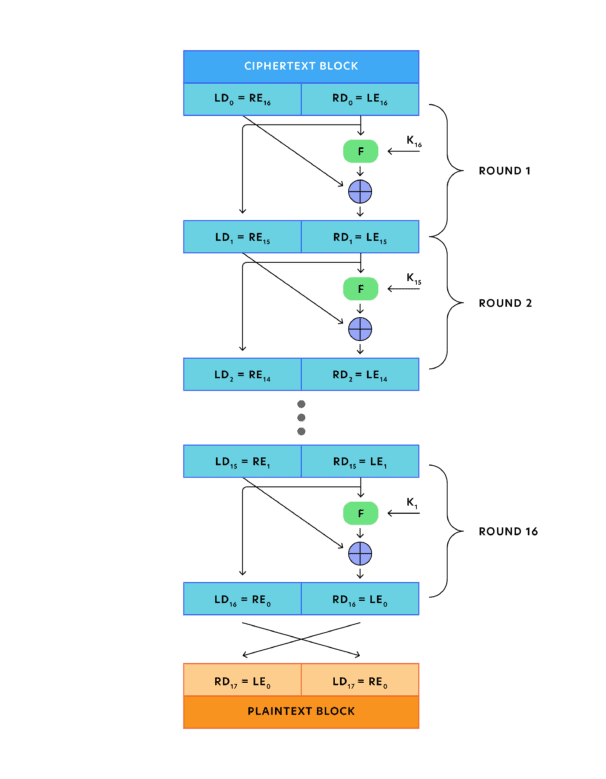
\includegraphics[scale=0.5]{fiestal_cipher.png}
	\caption{Fiestal Cipher Decryption Method}
\end{figure}


\section{Platform}
\textbf{Operating System}: Arch Linux x86-64 \\
\textbf{IDEs or Text Editors Used}: Visual Studio Code\\
\textbf{Compilers or Interpreters} : Python 3.10.1\\

\section{Input and Output}
\begin{verbatim}
    The plain text, key
    [1, 1, 1, 1, 0, 0, 1, 1] [1, 0, 1, 0, 0, 0, 0, 0, 1, 0]
    The left and right keys are :  [1, 0, 1, 0, 0, 1, 0, 0] [0, 1, 0, 0, 0, 0, 1, 1]
    Starting to cipher. 
    The cipher text is :  [0, 1, 0, 0, 0, 0, 0, 1]
\end{verbatim}
\section{Code}
\lstinputlisting[language=Python, caption="Fiestal Cipher"]{../Programs/Assignment_2/fiestel_cipher.py}

\section{Conclusion}
Thus, learnt about the different kinds of ciphers, classical cryptographic techniques, and how to implement some of them in python.
\clearpage

\section{FAQ}

\begin{enumerate}
	\item \textbf{Differentiate between stream and block ciphers.}\\
	      \begin{enumerate}
		      \item Stream ciphers encrypt the data one bit at a time. Block ciphers encrypt the data in blocks of fixed size.
		      \item Stream ciphers are faster than block ciphers.
		      \item Block ciphers are more secure than stream ciphers.
		      \item Stream ciphers are more suitable for real-time applications.
		      \item Block ciphers are more suitable for bulk data encryption.
		      \item Stream ciphers are more suitable for applications where the data is encrypted and decrypted in a single pass.
		      \item Block ciphers are more suitable for applications where the data is encrypted and decrypted in multiple passes.
	      \end{enumerate}

	\item \textbf{Write advantages and disadvantages of DES algorithm.}\\

	      \textbf{Advantages:}
	      \begin{enumerate}
		      \item It is a fast, simple, efficient, and secure algorithm.
		      \item The algorithm has been in use since 1977. Technically, no weaknesses have been found in the algorithm. Brute force attacks are still the most efficient attacks against the DES algorithm.
		      \item DES is the standard set by the US Government. The government recertifies DES every five years, and has to ask for its replacement if the need arises.
		      \item The American National Standards Institute (ANSI) and International Organization for Standardization (ISO) have declared DES as a standard as well. This means that the algorithm is open to the public—to learn and implement.
		      \item DES was designed for hardware; it is fast in hardware, but only relatively fast in software.
	      \end{enumerate}

	      \textbf{Disadvantages:}
	      \begin{enumerate}
		      \item Probably the biggest disadvantage of the DES algorithm is the key size of 56-bit. There are chips available that can encrypt and decrypt a million DES operations in a second. A DES cracking machine that can search all the keys in about seven hours is available for 1 million.
		      \item DES can be implemented quickly on hardware. But since it was not designed for software, it is relatively slow on it.
		      \item It has become easier to break the encrypted code in DES as the technology is steadily improving. Nowadays, AES is preferred over DES.
		      \item DES uses a single key for encryption as well as decryption as it is a type of symmetric encryption technique. In case that one key is lost, we will not be able to receive decipherable data at all.
	      \end{enumerate}

	\item \textbf{Explain block cipher modes of operations.}\\
	      \begin{enumerate}
		      \item \textit{Electronic Code Book (ECB)}
		            \begin{enumerate}
			            \item ECB mode stands for Electronic Code Block Mode. It is one of the simplest modes of operation. In this mode, the plain text is divided into a block where each block is 64 bits. Then each block is encrypted separately. The same key is used for the encryption of all blocks. Each block is encrypted using the key and makes the block of ciphertext.
			            \item At the receiver side, the data is divided into a block, each of 64 bits. The same key which is used for encryption is used for decryption. It takes the 64-bit ciphertext and, by using the key convert the ciphertext into plain text.
			            \item As the same key is used for all blocks’ encryption, if the block of plain text is repeated in the original message, then the ciphertext’s corresponding block will also repeat. As the same key used for tor all block, to avoid the repetition of block ECB mode is used for an only small message where the repetition of the plain text block is less.
		            \end{enumerate}

		            \begin{figure}[H]
			            \centering
			            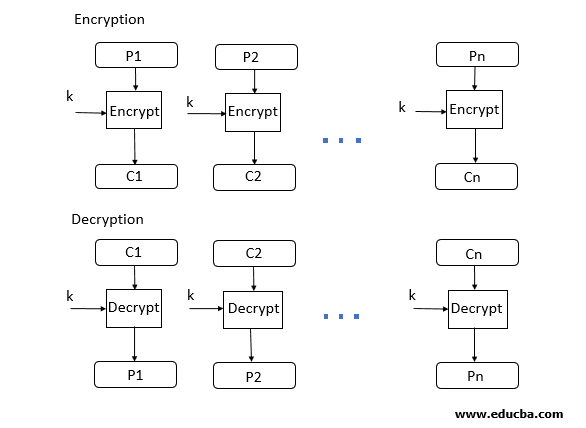
\includegraphics[scale=0.5]{ecb.jpg}
			            \caption{ECB Mode of Operation}
		            \end{figure}

		      \item \textit{Cipher Block Chaining (CBC)}
		            \begin{enumerate}
			            \item CBC Mode stands for Cipher block Mode at the sender side; the plain text is divided into blocks. In this mode, IV(Initialization Vector) is used, which can be a random block of text. IV is used to make the ciphertext of each block unique.
			            \item The first block of plain text and IV is combined using the XOR operation and then encrypted the resultant message using the key and form the first block of ciphertext. The first block of ciphertext is used as IV for the second block of plain text. The same procedure will be followed for all blocks of plain text.
			            \item At the receiver side, the ciphertext is divided into blocks. The first block ciphertext is decrypted using the same key, which is used for encryption. The decrypted result will be XOR with the IV and form the first block of plain text. The second block of ciphertext is also decrypted using the same key, and the result of the decryption will be XOR with the first block of ciphertext and form the second block of plain text. The same procedure is used for all the blocks.
			            \item CBC Mode ensures that if the block of plain text is repeated in the original message, it will produce a different ciphertext for corresponding blocks.
			                  Note that the key which is used in CBC mode is the same; only the IV is different, which is initialized at a starting point.
		            \end{enumerate}

		            \begin{figure}[H]
			            \centering
			            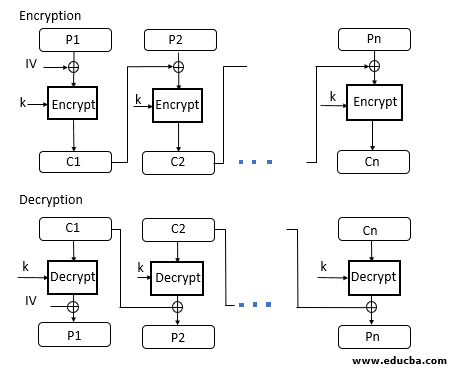
\includegraphics[scale=0.5]{cbc.jpg}
			            \caption{CBC Mode of Operation}
		            \end{figure}
		      \item \textit{Cipher Feedback (CFB)}

		            \begin{enumerate}
			            \item CFB mode stands for Cipher Feedback Mode. In this mode, the data is encrypted in the form of units where each unit is of 8 bits.
			            \item Like cipher block chaining mode, IV is initialized. The IV is kept in the shift register. It is encrypted using the key and form the ciphertext.
			            \item Now the leftmost j bits of the encrypted IV is XOR with the plain text’s first j bits. This process will form the first part of the ciphertext, and this ciphertext will be transmitted to the receiver.
			            \item Now the bits of IV is shifted left by j bit. Therefore the rightmost j position of the shift register now has unpredictable data. These rightmost j positions are now filed with the ciphertext. The process will be repeated for all plain text units.
		            \end{enumerate}

		            \begin{figure}[H]
			            \centering
			            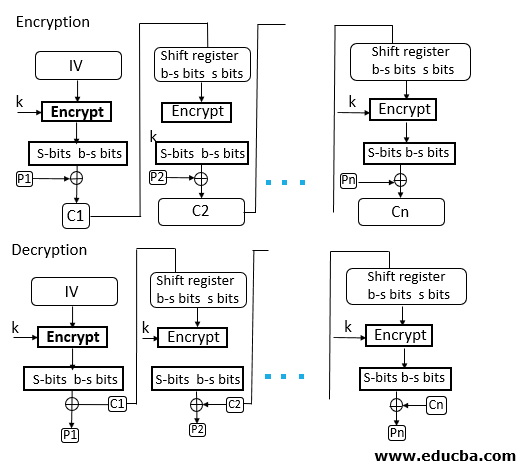
\includegraphics[scale=0.6]{cfb.jpg}
			            \caption{CFB Mode of Operation}
		            \end{figure}

		      \item \textit{Output Feedback (OFB)}

		            \begin{enumerate}
			            \item OFB Mode stands for output feedback Mode. OFB mode is similar to CFB mode; the only difference is in CFB, the ciphertext is used for the next stage of the encryption process, whereas in OFB, the output of the IV encryption is used for the next stage of the encryption process.
			            \item The IV is encrypted using the key and form encrypted IV. Plain text and leftmost 8 bits of encrypted IV are combined using XOR and produce the ciphertext.
			            \item For the next stage, the ciphertext, which is the form in the previous stage, is used as an IV for the next iteration. The same procedure is followed for all blocks.
		            \end{enumerate}

		            \begin{figure}[H]
			            \centering
			            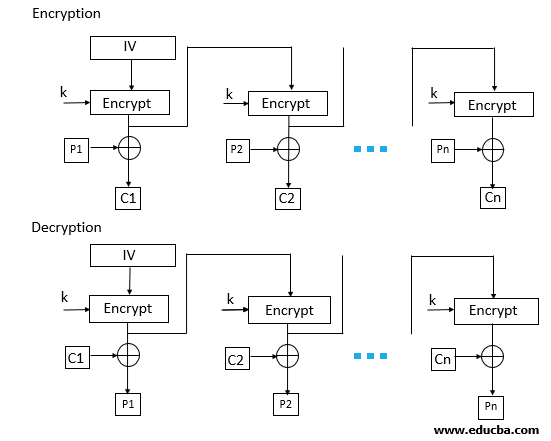
\includegraphics[scale=0.5]{ofm.jpg}
			            \caption{Output Feedback Mode of Operation}
		            \end{figure}
		      \item \textit{Counter (CTR)}

		            \begin{enumerate}
			            \item CTR Mode stands for counter mode. As the name is counter, it uses the sequence of numbers as an input for the algorithm. When the block is encrypted, to fill the next register next counter value is used.
			            \item For encryption, the first counter is encrypted using a key, and then the plain text is XOR with the encrypted result to form the ciphertext.
			            \item The counter will be incremented by 1 for the next stage, and the same procedure will be followed for all blocks. For decryption, the same sequence will be used. Here to convert ciphertext into plain text, each ciphertext is XOR with the encrypted counter. For the next stage, the counter will be incremented by the same will be repeated for all Ciphertext blocks.
		            \end{enumerate}

		            \begin{figure}[H]
			            \centering
			            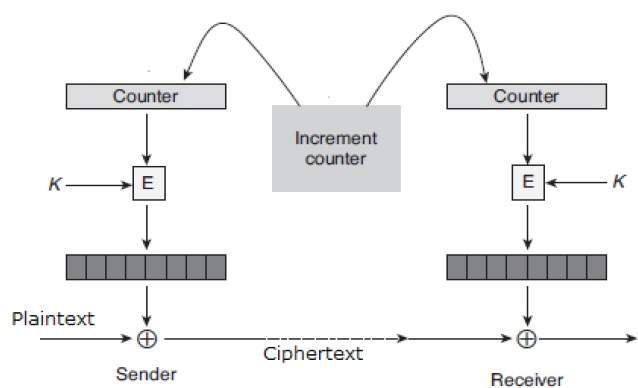
\includegraphics[scale=0.5]{ctr_mode.jpg}
			            \caption{}
		            \end{figure}
	      \end{enumerate}
\end{enumerate}


\chapter{S-AES Symmetric Key Algorithm}
\section{Aim}
Write a program using JAVA or Python or C++ to implement S-AES symmetric key
algorithm.

\section{Objectives}
To understand the concepts of block cipher and symmetric key cryptographic
system.

\section{Theory}

\subsection{What is Simplified AES?}
S-AES is to AES as S-DES is to DES. In fact, the structure of S-AES is exactly the
same as AES. The differences are in the key size (16 bits), the block size (16 bits) and the number
of rounds (2 rounds).

The Advanced Encryption Standard (AES) is a widely-used symmetric-key encryption algorithm that is used to encrypt and decrypt data. The simplified AES algorithm is a simplified version of the AES algorithm that is often used as a teaching tool to help people understand how AES works.

The simplified AES algorithm operates on a 4x4 matrix of bytes called a "state." The algorithm consists of several rounds, each of which performs a series of operations on the state. The number of rounds depends on the key size: 10 rounds for a 128-bit key, 12 rounds for a 192-bit key, and 14 rounds for a 256-bit key.

The simplified AES algorithm is a simplified version of the AES algorithm that is often used as a teaching tool to help people understand how AES works.


\begin{figure}[H]
	\centering
	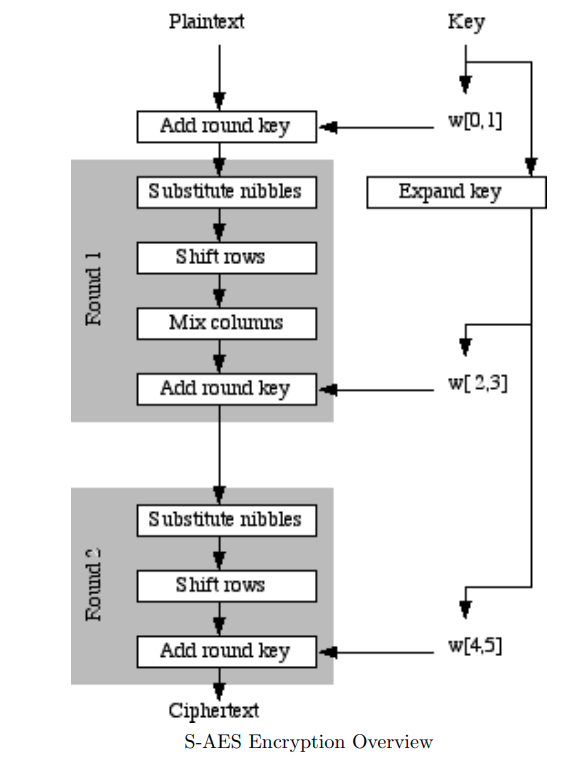
\includegraphics[scale=0.5]{saes.png}
	\caption{}
\end{figure}

\subsection{Key Expansion}
The key expansion function is the same as AES. The key is expanded to 32 bits and
then split into two 16-bit keys. The first key is used in the first round and the second key is used in the second round.
\subsection{Constants}

\subsection{Substitution}
In this step, each byte in the state is replaced by another byte using a substitution table called the S-box. The S-box is a fixed table that maps each possible byte value to another byte value. The byte value is used to look up a corresponding value in the S-box. The substitution is done in a byte-wise manner.
\subsection{Shift Rows}

% \subsection{Mix Columns}

% \subsection{Key Expansion Function (g())}

% \subsection{Round Function}

% \subsection{Encryption}

% \subsection{Decryption}

Here are the steps of one round of the simplified AES algorithm:

\begin{enumerate}
	\item SubBytes: In this step, each byte in the state is replaced by another byte using a substitution table called the S-box.

	\item ShiftRows: In this step, the bytes in each row of the state are shifted to the left. The first row is not shifted, the second row is shifted by one byte to the left, the third row is shifted by two bytes to the left, and the fourth row is shifted by three bytes to the left.

	\item MixColumns: In this step, each column of the state is multiplied by a fixed matrix. This is a bit more complex than the other steps, but it essentially "mixes" the bytes in each column.

	\item AddRoundKey: In this step, each byte in the state is XORed with a byte from the key schedule. The key schedule is derived from the original key using a key expansion algorithm.
\end{enumerate}

\section{Platform}
\textbf{Operating System}: Arch Linux x86-64 \\
\textbf{IDEs or Text Editors Used}: Visual Studio Code\\
\textbf{Compilers or Interpreters} : Python 3.10.1\\

\section{Input and Output}
\begin{verbatim}
    Enter Text to be encrypted via S-AES:AES is much better than DES
    Enter 4 digit Key to be used for encryption:9087
    Your Cipher Text is:  
                          HéWõëd¸½Kùд^#EGã'
    The decrypted plain text is:  AES is much better than DES
\end{verbatim}
\section{Code}
\lstinputlisting[language=Python, caption="Fiestal Cipher"]{../Programs/Assignment_3/Simplified_AES.py}

\section{Conclusion}
Thus, learnt about the different kinds of ciphers, classical cryptographic techniques, and how to implement some of them in python.
\clearpage

\section{FAQ}

\begin{enumerate}
	\item \textbf{Differentiate between DES and AES.}\\
	      \textbf{AES: }
	      \begin{enumerate}
		      \item AES stands for advanced encryption standard.
		      \item The key length can be 128 bits, 192 bits, or 256 bits.
		      \item The rounds of operations per key length are as follows: 128 bits: 10 192 bits: 12 256 bits: 14
		      \item AES is based on a substitution and permutation network.
		      \item AES is considered the standard encryption algorithm in the world and is more secure than DES.
		      \item Key Addition, Mix Column, Byte Substitution, and Shift Row.
		      \item AES can encrypt plaintext of 128 bits.
		      \item AES was derived from the Square Cipher.
		      \item AES was designed by Vincent Rijmen and Joan Daemen.
		      \item There are no known attacks for AES.
	      \end{enumerate}

	      \textbf{DES: }
	      \begin{enumerate}
		      \item DES stands for data encryption standard.
		      \item The key length is 56 bits.
		      \item There are 16 identical rounds of operations.
		      \item DES is based on the Feistel network.
		      \item DES is considered to be a weak encryption algorithm; triple DES is a more secure encryption algorithm.
		      \item Substitution, XOR Operation, Permutation, and Expansion.
		      \item DES can encrypt plaintext of 64 bits.
		      \item DES was derived from the Lucifer Cipher.
		      \item DES was designed by IBM.
		      \item Brute force attacks, differential cryptanalysis, and linear cryptanalysis.
	      \end{enumerate}

	\item \textbf{What are the different advantages and Limitations of AES?}\\
	      \textbf{Advantages: }\\
	      \begin{enumerate}
		      \item Following are the benefits or advantages of AES:
		      \item As it is implemented in both hardware and software, it is most robust security protocol.
		      \item It uses higher length key sizes such as 128, 192 and 256 bits for encryption. Hence it makes AES algorithm more robust against hacking.
		      \item It is most common security protocol used for wide various of applications such as wireless communication, financial transactions, e-business, encrypted data storage etc.
		      \item It is one of the most spread commercial and open source solutions used all over the world.
		      \item No one can hack your personal information.
		      \item For 128 bit, about 2128 attempts are needed to break. This makes it very difficult to hack it as a result it is very safe protocol.
	      \end{enumerate}


	      \textbf{Limitations: }\\
	      \begin{enumerate}
		      \item It uses too simple algebraic structure.
		      \item Every block is always encrypted in the same way.
		      \item Hard to implement with software.
		      \item AES in counter mode is complex to implement in software taking both performance and security into considerations.
	      \end{enumerate}

\end{enumerate}



\chapter{RSA Asymmetric Key Algorithm}
\section{Aim}
Write a program using JAVA or Python or C++ to implement RSA asymmetric key
algorithm.

\section{Objectives}
To understand the concepts of public key and private key

\section{Theory}

\subsection{Euler Totient Function}
Euler's Totient function, denoted as $\varphi(n)$, is a number theoretic function that counts the number of positive integers less than or equal to $n$ that are relatively prime to $n$. In other words, $\varphi(n)$ gives the number of integers in the range $1 \leq k \leq n$ such that $\gcd(k, n) = 1$.

Here is an example of how to calculate Euler's Totient function for a specific integer $n$:

Let's take $n = 12$. The prime factorization of $n$ is $n = 2^2 \cdot 3^1$, so we can use the formula for calculating $\varphi(n)$ in terms of the prime factorization of $n$:

$$\varphi(n) = n \cdot \prod_{p \mid n} \left(1 - \frac{1}{p}\right)$$

where the product is taken over all distinct prime factors of $n$. Plugging in the prime factorization of $n = 12$, we get:

\begin{align*}
\varphi(12) &= 12 \cdot \left(1 - \frac{1}{2}\right) \cdot \left(1 - \frac{1}{3}\right) \\
&= 12 \cdot \frac{1}{2} \cdot \frac{2}{3} = 4
\end{align*}

Therefore, the value of Euler's Totient function for $n = 12$ is $\varphi(12) = 4$. This means that there are 4 positive integers less than or equal to 12 that are relatively prime to 12: 1, 5, 7, and 11.

\subsection{Euclidean Algorithm}
The Euclidean Algorithm is a method for finding the greatest common divisor (GCD) of two integers. It works by repeatedly finding the remainder when one integer is divided by the other, and then replacing the larger integer with the remainder. This process is repeated until the remainder is zero, at which point the GCD is the last non-zero remainder.

Here is an example of the Euclidean Algorithm applied to finding the GCD of 54 and 24:

\begin{align*}
	54 & = 2 \cdot 24 + 6 \\
	24 & = 4 \cdot 6 + 0 \
\end{align*}

We start by dividing 54 by 24 and finding the remainder, which is 6. We then replace 54 with 24 and 24 with 6, and repeat the process by dividing 24 by 6 and finding the remainder, which is 0. Since the remainder is now zero, the GCD is the last non-zero remainder, which in this case is 6. Therefore, the GCD of 54 and 24 is 6.

\subsection{Extended Euclidean Algorithm}
The Extended Euclidean Algorithm is an extension of the Euclidean Algorithm that not only finds the GCD of two integers, but also finds two coefficients that can be used to express the GCD as a linear combination of the two integers. Specifically, given two integers $a$ and $b$, the Extended Euclidean Algorithm finds integers $x$ and $y$ such that:

$$ax + by = \gcd(a, b)$$

Here is an example of the Extended Euclidean Algorithm applied to finding the GCD of 54 and 24, along with the coefficients $x$ and $y$:

\begin{align*}
	54 & = 2 \cdot 24 + 6 \\
	24 & = 4 \cdot 6 + 0 \
\end{align*}

To start, we apply the Euclidean Algorithm as we did before to find the GCD of 54 and 24, which is 6. We then work backwards through the steps of the algorithm to find the coefficients $x$ and $y$.

Starting from the second-to-last step:

\begin{align*}
	6 & = 54 - 2 \cdot 24 \
\end{align*}

We can rearrange this equation to isolate 6:

\begin{align*}
	6 & = 54 - 2 \cdot 24 \\
	  & = 54 - 2(54 - 2 \cdot 24) \\
	  & = 5 \cdot 54 - 2 \cdot 24
\end{align*}

So, we have found that $x = 5$ and $y = -2$. Substituting these values into the original equation, we get:

\begin{align*}
	54(5) + 24(-2) & = 6 \
\end{align*}

Therefore, the GCD of 54 and 24 is 6, and it can be expressed as a linear combination of 54 and 24 with coefficients 5 and -2, respectively.

\subsection{RSA Algorithm}
\subsubsection{Key Generation}
\begin{enumerate}
	\item Selecting two large primes at random: $p$ and $q$.
	\item Computing their system modulus: $n = (p*q)$.
	\item Compute: $\phi(n) = (p-1)*(q-1)$.
	\item selecting at random the encryption key (public key): $e$ such that $1 < e < \phi(n)$ and $gcd(e, \phi(n)) = 1$.
	\item To find decryption key d such that $d*e \equiv 1 \pmod{\phi(n)}$.
	\item Public Encryption key: $PU = {e, n}$
	\item Private Decryption key: $PR = {d, n}$
\end{enumerate}
\subsubsection{RSA Encryption}
Encrypt the plain text $M$ using the public key $PU$.
\begin{enumerate}
	\item Computes Cipher text: $C = M^e \pmod{n}$, where 0 <= $M$ < $n$.
\end{enumerate}

\subsubsection{RSA Decryption}
Decrypt the cipher text $C$ using the private key $PR$.
\begin{enumerate}
	\item Computes Plaintext: $M = C^d \pmod{n}$
\end{enumerate}

\subsubsection{Example of RSA Encryption}
\begin{enumerate}
	\item Select two large primes at random: $p = 3$ and $q = 11$.
	\item Compute their system modulus: $n = (p*q) = 33$.
	\item Compute: $\phi(n) = (p-1)*(q-1) = 20$.
	\item Select at random the encryption key (public key): $e = 7$ such that $1 < e < \phi(n)$ and $gcd(e, \phi(n)) = 1$.
	\item To find decryption key d such that $d*e \equiv 1 \pmod{\phi(n)}$.
	\item Public Encryption key: $PU = {e, n} = {7, 33}$
	\item Private Decryption key: $PR = {d, n} = {3, 33}$
	\item Encrypt the plain text $M = 30$ using the public key $PU$.
	\item Computes Cipher text: $C = M^e \pmod{n} = 5^7 \pmod{33} = 24$.
	\item Decrypt the cipher text $C = 24$ using the private key $PR$.
	\item Computes Plaintext: $M = C^d \pmod{n} = 24^3 \pmod{33} = 30$.
\end{enumerate}

\section{Platform}
\textbf{Operating System}: Arch Linux x86-64 \\
\textbf{IDEs or Text Editors Used}: Visual Studio Code\\
\textbf{Compilers or Interpreters} : Python 3.10.1\\

\section{Input and Output}
\begin{verbatim}
Enter the Message to be encrypted: 
This Assignment's Due date is very near
private key is:  (14633, 31373)
public key is:  (89, 31373)
<encrypted text>
This Assignment's Due date is very near
\end{verbatim}
\section{Code}
\lstinputlisting[language=Python, caption="RSA Algorithm"]{../Programs/Assignment_4/rsa.py}

\section{Conclusion}
Thus, learnt about the different kinds of public key cryptography works. Also, learnt about the RSA algorithm and its implementation in Python in depth. We also tried to implement RSA on a dummy client server model using sockets in python.
\clearpage

\section{FAQ}

\begin{enumerate}
	\item \textit{Compare symmetric key cryptography and asymmetric key cryptography}\\
	
	      \begin{enumerate}
		      \item \textit{Symmetric Key Cryptography}
		            \begin{itemize}
			            \item \textit{Advantages}
			                  \begin{itemize}
				                  \item \textit{Fast}
				                  \item \textit{Easy to implement}
				                  \item \textit{Easy to share the key}
			                  \end{itemize}
			            \item \textit{Disadvantages}
			                  \begin{itemize}
				                  \item \textit{Key Distribution is a problem}
				                  \item \textit{Key Management is a problem}
			                  \end{itemize}
		            \end{itemize}
		      \item \textit{Asymmetric Key Cryptography}
		            \begin{itemize}
			            \item \textit{Advantages}
			                  \begin{itemize}
				                  \item \textit{Easy to share the key}
				                  \item \textit{Easy to manage the key}
			                  \end{itemize}
			            \item \textit{Disadvantages}
			                  \begin{itemize}
				                  \item \textit{Slow}
				                  \item \textit{Difficult to implement}
			                  \end{itemize}
		            \end{itemize}
	      \end{enumerate}

	\item \textit{Write advantages and disadvantages of RSA algorithm.}\\
	
	      \textbf{Advantages}
	      \begin{itemize}
		      \item \textit{RSA is a public key algorithm} : The public key is available to everyone. The private key is kept secret. The public key is used for encryption and the private key is used for decryption.
		      \item \textit{RSA is a secure algorithm} : The security of RSA is based on the difficulty of factoring large integers. The security of RSA depends on the fact that the factoring of the product of two large prime numbers is difficult. This is to say that it is a very difficult problem to find the two prime factors of a large composite number, and therefore it makes RSA very secure.
		      \item \textit{RSA is a widely used algorithm} : RSA is used in many applications such as secure email, digital signatures, file encryption, etc.
	      \end{itemize}
	      \textbf{Disadvantages}
	      \begin{itemize}
		      \item \textit{RSA is a slow algorithm} : The RSA algorithm is slow because of the large number of multiplications and modular exponentiations that are required.
		      \item \textit{RSA is not suitable for bulk data encryption} : RSA is not suitable for bulk data encryption because of its slowness. It is suitable for encrypting small amounts of data.
	      \end{itemize}
\end{enumerate}



\chapter{Integrity of Message using MD5 or SHA}
\section{Aim}
Write a program using JAVA or Python or C++ to implement integrity of message using
MD5 or SHA

\section{Objectives}
To use of hashing algorithm to check message integrity.

\section{Theory}

\subsection{Secure Hashing Algorithm (SHA-256)}

\begin{figure}[H]
    \centering
    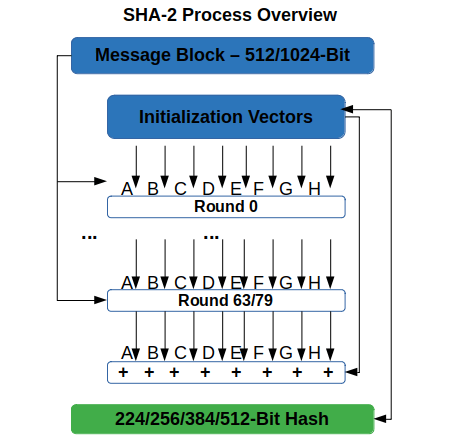
\includegraphics[width=0.55\textwidth]{how-the-sha2-hashing-algorithm-works.png}
    \caption{Working of SHA-256}
\end{figure}

\textit{SHA-256 is a widely used cryptographic hash function that generates a 256-bit (32-byte) digest or hash value from an input message.}

Here are the steps involved in the SHA-256 algorithm:

\begin{enumerate}
    \item \textbf{Message padding}: The input message is padded so that its length is a multiple of 512 bits, which is the block size used by SHA-256. The padding scheme used by SHA-256 is similar to the one used by SHA-1, but with some modifications.

    \item \textbf{Initialize hash values}: SHA-256 uses eight initial hash values, represented as 32-bit words. These values are specified in the SHA-256 specification and are typically denoted as H0, H1, H2, H3, H4, H5, H6, and H7.

    \item \textbf{Process message in 512-bit blocks}: The padded message is divided into 512-bit blocks, and each block is processed by the SHA-256 algorithm.

    \item \textbf{Initialize working variables}: SHA-256 uses a set of working variables, represented as 32-bit words, to store intermediate values during the hashing process. These working variables are typically denoted as a, b, c, d, e, f, g, and h.

    \item \textbf{Compute the hash}: For each 512-bit block, SHA-256 performs 64 rounds of computation to update the working variables and generate the hash value. Each round involves several operations, including bitwise operations, logical operations, and modular addition. The specific operations used in SHA-256 are designed to provide strong cryptographic properties, such as collision resistance and preimage resistance.

    \item \textbf{Combine hash values}: After processing all blocks in the message, the final hash value is computed by combining the eight 32-bit hash values computed during the process. This is typically done by concatenating the hash values in the order H0, H1, H2, H3, H4, H5, H6, and H7 to obtain the 256-bit SHA-256 digest.
\end{enumerate}

\subsection{Example}

\begin{enumerate}
    \item here is an example of how SHA-256 can be used to generate a hash value from a sample input message "Hello, world!":

    \item \textbf{Message Padding}: The ASCII encoding of the message is "48656c6c6f2c20776f726c6421". To pad the message to a length that is a multiple of 512 bits, the message is first appended with a single "1" bit, followed by as many "0" bits as necessary to make the length of the message 448 bits (56 bytes less than a multiple of 512). Then, the original length of the message in bits (80 bits in this case) is added as a 64-bit big-endian integer. Therefore, the padded message is:

          48656c6c6f2c20776f726c64210000000000000000000000000000000000000000000\\
          00000000000000000000005000

    \item \textbf{Initialize Hash Values}: The initial hash values for SHA-256 are specified in the SHA-256 specification and are typically denoted as H0, H1, H2, H3, H4, H5, H6, and H7:

          H0 = 6a09e667
          H1 = bb67ae85
          H2 = 3c6ef372
          H3 = a54ff53a
          H4 = 510e527f
          H5 = 9b05688c
          H6 = 1f83d9ab
          H7 = 5be0cd19

    \item \textbf{Process Message in 512-bit Blocks}: The padded message is divided into 512-bit blocks, and each block is processed by the SHA-256 algorithm. In this case, there is only one block since the message is short enough to fit into a single block.

    \item \textbf{Initialize Working Variables}: SHA-256 uses a set of working variables, represented as 32-bit words, to store intermediate values during the hashing process. These working variables are typically denoted as a, b, c, d, e, f, g, and h:

          a = H0
          b = H1
          c = H2
          d = H3
          e = H4
          f = H5
          g = H6
          h = H7

    \item \textbf{Compute the Hash}: For each 512-bit block, SHA-256 performs 64 rounds of computation to update the working variables and generate the hash value. Each round involves several operations, including bitwise operations, logical operations, and modular addition. Here is a summary of the operations for the first block:

    \item \textbf{Divide the block into 16 32-bit words, denoted as W[0] through W[15]}:
          Compute W[i] for i from 16 to 63 using the formula: sigma1(W[i-2]) + W[i-7] + sigma0(W[i-15]) + W[i-16], where sigma0 and sigma1 are specific bitwise operations used in SHA-256.
          Initialize temporary variables T1 and T2 to a and e, respectively.
          Perform 64 rounds of computation using the formulae:
          T1 = h + Sigma1(e) + Ch(e, f, g) + K[i] + W[i]
          T2 = Sigma0(a) + Maj(a, b, c)

    \item \textbf{Finalize Hash Value}: After processing all of the blocks, the final hash value is computed by concatenating the values of a, b, c, d, e, f, g, and h, in that order, and converting each 32-bit word to a 4-byte big-endian integer. In this example, the final hash value is:

          0x7cf5d5e440b5d760b5a22d9b759f4419f544e1e7525ccae037ba20a8d1e26c35
\end{enumerate}


\section{Platform}
\textbf{\textbf{Operating System}}: Arch Linux x86-64 \\
\textbf{\textbf{IDEs or Text Editors Used}}: Visual Studio Code\\
\textbf{\textbf{Compilers or Interpreters} }: Python 3.10.1\\

\section{Input and Output}

\subsection*{Image Before Changing}
\begin{figure}[H]
    \centering
    
\includegraphics[width=.90\textwidth]{tony.jpg}
    \caption{Tony Stark Just before Showcasing the Jericho Missile}
\end{figure}
\subsection*{Image After Changing}
\begin{figure}[H]
    \centering
    
\includegraphics[width=.90\textwidth]{tony_changed.jpg}
    \caption{Tony Stark Just before Showcasing the Jericho Missile, but with a hidden message}
\end{figure}

\begin{verbatim}
Hash of the file is: 
b91bf2a1dd825725f788a7e204cfd38d0a4badd1bf3745ec2efceeb4e3cab591
Modified the File, added hidden data to it.
Data: I am Iron Man and I love by daughter 3000.
Hash of the file now is: 
d02d021cc9c7771339327216c82540b1796ce1f2d715797907c97ee7c24788e8
\end{verbatim}


\section{Code}
\lstinputlisting[language=Python, caption="SHA Integrity Check"]{../Programs/Assignment_5/sha.py}

\section{Conclusion}
Thus, learnt about the different types of message integrity checks and how to implement them in Python.
MD5 and SHA are the most commonly used message integrity checks, and were implemented in this assignment using the hashlib library.

\clearpage

\section{FAQ}

\begin{enumerate}
    \item \textit{What is MAC? What is the difference between MAC and message digest.} \\

          \textbf{\textbf{Definition}}: \\

          \textbf{MAC} stands for \textit{Message Authentication Code}, and it is \textit{a type of cryptographic technique used to provide integrity and authenticity of a message.} A MAC is generated by taking a secret key and combining it with the message using a cryptographic hash function or a symmetric encryption algorithm. The resulting MAC is appended to the message and sent along with it. The receiver can then use the same secret key and cryptographic algorithm to compute the MAC and verify that it matches the MAC sent with the message, thus ensuring the integrity and authenticity of the message.

          A \textbf{message digest}, on the other hand, is \textit{a fixed-length output generated by applying a cryptographic hash function to a message.} The resulting digest can be used to verify that the message has not been tampered with, but it does not provide authentication. A message digest can be thought of as a digital fingerprint of a message, which is unique to that message and can be used to identify any changes made to the message.\\


          \textbf{Differences}:\\

          \begin{enumerate}
              \item \textbf{Purpose}: The purpose of MAC is to provide both integrity and authenticity of a message, while the purpose of a message digest is to provide integrity only.

              \item \textbf{Technique}: MAC uses a secret key and a cryptographic algorithm such as a hash function or a symmetric encryption algorithm to create a unique code that authenticates the message. In contrast, message digest only uses a cryptographic hash function to generate a fixed-length output that verifies the integrity of the message.

              \item \textbf{Key Requirements}: MAC requires a secret key that is shared between the sender and receiver to generate the code, while message digest only requires a publicly available cryptographic hash function.

              \item \textbf{Strength}: MAC provides stronger authentication than message digest because it uses a secret key to create a unique code that cannot be forged. Message digest, on the other hand, only provides integrity verification and can be more susceptible to attacks.

              \item \textbf{Resource Requirements}: MAC requires more computational resources than message digest because it uses a cryptographic algorithm that requires more processing power. Additionally, MAC requires a secure key distribution channel, which can add to the resource requirements.

              \item \textbf{Usage}: MAC is commonly used in secure communication protocols such as SSL/TLS, IPSec, and SSH, while message digest is commonly used for verifying file integrity, password storage, and digital signatures.
          \end{enumerate}


    \item \textit{Compare MD5 and SHA-1.} \\
          MD5 and SHA1 are both cryptographic hash functions that are used to generate a fixed-length output, or digest, from a message. Here are some differences between MD5 and SHA1:

          \begin{enumerate}
              \item \textbf{Output size}: MD5 generates a 128-bit digest, while SHA1 generates a 160-bit digest. This means that SHA1 is slightly stronger than MD5 in terms of the number of possible output values.

              \item \textbf{Collision resistance}: MD5 is considered to be weak in terms of collision resistance, which means that it is possible to generate two different messages that produce the same MD5 digest. SHA1 is also vulnerable to collision attacks, but it is considered to be stronger than MD5.

              \item \textbf{Speed}: MD5 is generally faster than SHA1 because it uses a simpler algorithm. However, because of its weaknesses, it is no longer recommended for use in security-sensitive applications. SHA1 is slightly slower than MD5 but is still considered to be a fast and efficient hash function.

              \item \textbf{Usage}: MD5 was once widely used in security applications such as digital signatures and password storage, but it is now considered to be insecure and should be avoided. SHA1 is still commonly used for data integrity and message authentication, but it is gradually being phased out in favor of stronger hash functions such as SHA-256 and SHA-3.

              \item \textbf{Security}: Both MD5 and SHA1 are considered to be weak and vulnerable to attacks by modern computing resources, which can compromise their security in practical applications. As a result, it is recommended to use stronger cryptographic hash functions, such as SHA-256 or SHA-3, for security-sensitive applications.
          \end{enumerate}

    \item \textit{Compare various versions of SHA.} \\

          There are several versions of the SHA (Secure Hash Algorithm) family of cryptographic hash functions, each with different strengths and output sizes. Here is a comparison of some of the most widely used SHA versions:

          \begin{enumerate}
              \item \textbf{SHA-1}: SHA-1 is a 160-bit hash function that was widely used for data integrity and message authentication. However, it is now considered to be vulnerable to collision attacks and has been deprecated in favor of stronger hash functions.

              \item \textbf{SHA-2}: SHA-2 is a family of hash functions that includes SHA-224, SHA-256, SHA-384, and SHA-512, each with different output sizes. SHA-256 is a 256-bit hash function that is widely used for digital signatures, file verification, and other security applications. SHA-384 and SHA-512 are designed for use in applications that require a higher level of security, such as secure communications and financial transactions.

              \item \textbf{SHA-3}: SHA-3 is the latest addition to the SHA family of hash functions, and was developed as a result of the NIST hash function competition. It is a family of hash functions that includes SHA3-224, SHA3-256, SHA3-384, and SHA3-512, each with different output sizes. SHA-3 is designed to be more secure and efficient than previous versions of SHA.

          \end{enumerate}

          \begin{enumerate}
              \item \textbf{Output size}: SHA-1 generates a 160-bit digest, SHA-2 generates a range of digest sizes from 224 to 512 bits, while SHA-3 also generates a range of digest sizes from 224 to 512 bits. Generally, larger output sizes provide stronger security and are more resistant to collision attacks.

              \item \textbf{Collision resistance}: SHA-1 has been found to be vulnerable to collision attacks, while SHA-2 and SHA-3 are designed to be more resistant to such attacks. SHA-3 is particularly strong in this regard due to its sponge construction.

              \item \textbf{Algorithm}: SHA-1, SHA-2, and SHA-3 all use different algorithms to generate their digests. SHA-1 and SHA-2 use a Merkle-Damgård construction, while SHA-3 uses a sponge construction. The sponge construction provides better resistance against attacks, such as length extension attacks, that can affect Merkle-Damgård construction.

              \item \textbf{Performance}: SHA-2 and SHA-3 generally require more processing power than SHA-1 due to their larger digest sizes and more complex algorithms. However, the performance difference may be insignificant in practice, and the security benefits of using SHA-2 or SHA-3 may outweigh the performance costs.

              \item \textbf{Standardization}: SHA-1 and SHA-2 are widely standardized and have been widely used in various security applications, while SHA-3 is a relatively new standard and has yet to gain widespread adoption.

              \item \textbf{Security}: SHA-1 is now considered insecure and should not be used in security-sensitive applications. SHA-2 and SHA-3 are considered to be secure and are recommended for use in security-sensitive applications, with SHA-3 being the stronger choice.
          \end{enumerate}


\end{enumerate}



\chapter{Diffie Hellman Key Exchange Algorithm}
\section{Aim}
Write a program using JAVA or Python or C++ to implement Diffie-Hellman Key Exchange Algorithm

\section{Objectives}
To learn how to distribute the key.

\section{Theory}

\subsection{What is the Diffie-Hellman Key Exchange Algorithm?}

Diffie-Hellman key exchange is a cryptographic protocol that allows two parties to establish a shared secret key over an insecure communication channel without any prior knowledge of each other. The protocol is based on the discrete logarithm problem and modular arithmetic, and it is widely used in secure communication systems such as SSL/TLS, VPNs, and SSH.

\subsection{Working of the Algorithm}

Here's how the Diffie-Hellman key exchange works, using a simple example:

\begin{enumerate}
    \item Alice and Bob agree on a large prime number p and a primitive root of p, g. These values are public and can be shared over an insecure channel.
    \item Alice chooses a random secret number a and computes $ A = g^a $ mod p. She sends A to Bob over the insecure channel.
    \item Bob chooses a random secret number b and computes $B = g^b$ mod p. He sends B to Alice over the insecure channel.
    \item Alice computes the shared secret key as $K = B^a$ mod p.
    \item Bob computes the shared secret key as $K = A^b$ mod p.
\end{enumerate}

\begin{figure}[H]
    \centering
    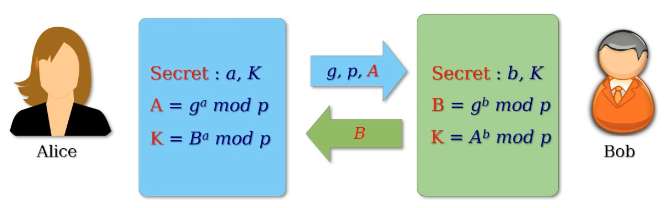
\includegraphics[width=.85\textwidth]{dh.png}
    \caption{Diffie Hellman Protocol}
\end{figure}

Both Alice and Bob end up with the same shared secret key K, which can be used for further encryption and decryption of messages.

\subsection{Example}
Alice and Bob agree on a large prime number $p=11$ and a primitive root of $p$, $g=2$. These values are public and can be shared over an insecure channel.

\begin{enumerate}
    \item Alice chooses a random secret number $a=7$ and computes $A = g^a \bmod p = 2^7 \bmod 11 = 7$. She sends $A=7$ to Bob over the insecure channel.
    \item Bob chooses a random secret number $b=5$ and computes $B = g^b \bmod p = 2^5 \bmod 11 = 10$. He sends $B=10$ to Alice over the insecure channel.
    \item Alice receives $B=10$ from Bob and computes the shared secret key as $K = B^a \bmod p = 10^7 \bmod 11 = 7$.
    \item Bob receives $A=7$ from Alice and computes the shared secret key as $K = A^b \bmod p = 7^5 \bmod 11 = 10$.
\end{enumerate}

Now Alice and Bob both have the same shared secret key $K=7=10$, which they can use to encrypt and decrypt their messages using a symmetric encryption algorithm such as AES.




\section{Platform}
\textbf{\textbf{Operating System}}: Arch Linux x86-64 \\
\textbf{\textbf{IDEs or Text Editors Used}}: Visual Studio Code\\
\textbf{\textbf{Compilers or Interpreters} }: Python 3.10.1\\

\section{Input and Output}

\begin{verbatim}
p:  239
g:  7
Shared secret key from A 95
Shared secret key from B 95
\end{verbatim}


\section{Code}
\lstinputlisting[language=Python, caption="SHA Integrity Check"]{../Programs/Assignment_6/diffie_hellman.py}

\section{Conclusion}
Thus, we have successfully implemented the Diffie-Hellman Key Exchange Algorithm. We learnt about the working of the algorithm and how it is used to distribute any key between 2 parties.
\clearpage

\section{FAQ}

\begin{enumerate}
    \item \textbf{What are other key exchange protocols, other than DH algorithm?}

          \begin{enumerate}
              \item \textbf{RSA Key Exchange}: This protocol uses the RSA algorithm to exchange keys securely between two parties.
              \item \textbf{Elliptic Curve Diffie-Hellman (ECDH)}: This is a variant of the DH algorithm that uses elliptic curve cryptography to provide stronger security and more efficient key exchange.
              \item \textbf{Kerberos}: This is a network authentication protocol that uses a trusted third party (a Key Distribution Center or KDC) to distribute secret keys between two parties.
              \item \textbf{Secure Remote Password (SRP)}: This is a password-based key exchange protocol that allows two parties to establish a shared secret key without revealing their passwords to each other or to an eavesdropper.
              \item \textbf{Signal Protocol}: This is a modern and widely used protocol for secure messaging that uses a combination of the Double Ratchet Algorithm and the DH algorithm to perform key exchange.
              \item \textbf{Station-to-Station (STS)}: This is a protocol that combines elements of the DH and RSA key exchange protocols to provide stronger security and more efficient key exchange.
          \end{enumerate}

    \item \textbf{Explain the different types of keys.}\\

          In cryptography, keys refer to the secret values used for encryption and decryption of messages.

          \begin{enumerate}

              \item \textbf{Symmetric Keys}: Also known as shared keys, these are secret keys that are used for both encryption and decryption of messages. The same key is used by both the sender and the receiver. Examples of symmetric key algorithms include AES, DES, and Blowfish.

              \item \textbf{Public Keys}: Also known as asymmetric keys, these are key pairs consisting of a public key and a private key. The public key is widely distributed and is used for encryption, while the private key is kept secret and is used for decryption. Examples of public key algorithms include RSA, Diffie-Hellman, and elliptic curve cryptography.

              \item \textbf{Session Keys}: These are temporary symmetric keys that are generated for a single session of communication between two parties. They are used to encrypt and decrypt messages exchanged during the session and are discarded once the session is over. Session keys are often used to provide forward secrecy, which means that compromising one session's key does not compromise the security of past or future sessions.

              \item \textbf{Key Exchange Keys}: These are public keys used specifically for exchanging symmetric keys between two parties. Key exchange algorithms like Diffie-Hellman and Elliptic Curve Diffie-Hellman are used to establish a shared secret key between two parties without actually transmitting the key over the communication channel.

          \end{enumerate}

    \item \textbf{Explain different key management issues.}\\

          Key management is the process of securely generating, storing, distributing, and revoking cryptographic keys. Here are some of the most common key management issues in cryptography:

          \begin{enumerate}
              \item \textbf{Key Generation}: The process of generating strong cryptographic keys is essential to ensuring the security of cryptographic systems. However, generating keys that are both random and unpredictable can be difficult. Key generation must be done securely, and the keys must be protected from disclosure or compromise.

              \item \textbf{Key Storage}: Cryptographic keys must be securely stored to prevent unauthorized access or disclosure. The storage of keys is often the weakest link in key management. Keys must be stored in a secure environment, and access to the keys must be tightly controlled.

              \item \textbf{Key Distribution}: Cryptographic keys must be securely distributed to all parties involved in the communication. Key distribution can be challenging, especially when there are multiple parties involved. Key exchange protocols like Diffie-Hellman and RSA can be used to securely exchange keys between parties.

              \item \textbf{Key Revocation}: Keys must be revoked when they are no longer needed or when they have been compromised. Revocation is necessary to prevent unauthorized access to data that was encrypted using the compromised key. Revocation can be challenging, especially in large systems where there are many keys in use.

              \item \textbf{Key Expiration}: Cryptographic keys have a limited lifespan, and must be periodically updated or replaced to maintain their security. Key expiration policies must be carefully designed to balance security and usability.

          \end{enumerate}

\end{enumerate}



\chapter{Digital signature using DSA}

\section{Aim}
Write a program using JAVA or Python or C++ to implement Digital signature using DSA

\section{Objectives}
To learn authentication technique for access control

\section{Theory}

\subsection{The Digital Signature Algorithm (DSA)}

The Digital Signature Algorithm (DSA) is a public key cryptographic algorithm that is used to create and verify digital signatures. It was developed by the US National Institute of Standards and Technology (NIST) and is based on the mathematical concept of modular exponentiation.

The DSA algorithm consists of three main components: key generation, signature generation, and signature verification.

\subsection{Algorithm}

\subsubsection{Key Generation:}

\begin{enumerate}
    \item Choose a prime number $p$ such that $p$ is 1024 bits or longer, and $p-1$ is divisible by a 160-bit prime number $q$.
    \item Choose an integer $g$ such that $1 < g < p$ and $g^{(p-1)/q} \bmod p \neq 1$.
    \item Choose a random integer $x$ such that $0 < x < q$.
    \item Compute $y = g^x \bmod p$.
    \item The public key is $(p, q, g, y)$, and the private key is $x$.
\end{enumerate}

\subsubsection{Signature Generation:}

\begin{enumerate}
    \item Choose a random integer $k$ such that $0 < k < q$.
    \item Compute $$r = (g^k \bmod p) \bmod q$$
    \item Compute $$s = k^{-1} (H(m) + xr) \bmod q$$ where $H(m)$ is the hash of the message $m$.
    \item The signature is $(r, s)$.
\end{enumerate}

\subsubsection{Signature Verification:}

\begin{enumerate}
    \item Verify that $0 < r < q$ and $0 < s < q$.
    \item Compute $w = s^{-1} \bmod q$.
    \item Compute $$u_1 = (H(m)w) \bmod q$$ and $$u_2 = (rw) \bmod q$$
    \item Compute $$v = ((g^{u_1} y^{u_2}) \bmod p) \bmod q$$
    \item If $v = r$, the signature is valid. Otherwise, it is invalid.
\end{enumerate}

\subsection{Example}

Here is an example of how the DSA algorithm works:

Suppose Alice wants to send a message to Bob and sign it using DSA. Alice and Bob have already generated their public and private keys.

\subsubsection{Signature Generation:}

\begin{enumerate}
    \item Alice chooses a random integer $k = 123$.
    \item Alice computes $$r = (g^k \bmod p) \bmod q = (2^{123} \bmod 467) \bmod 61 = 8$$
    \item Alice computes $$s = k^{-1} (H(m) + xr) \bmod q = 123^{-1} (H(m) + 22 \cdot 8) \bmod 61$$ where $H(m)$ is the hash of the message $m$.
    \item Alice sends the message and the signature $(r, s)$ to Bob.
\end{enumerate}

\subsubsection{Signature Verification:}

\begin{enumerate}
    \item Bob receives the message and the signature $(r, s)$ from Alice.
    \item Bob verifies that $0 < r < q$ and $0 < s < q$.
    \item Bob computes $$w = s^{-1} \bmod q = 123^{-1} \bmod 61 = 31$$
    \item Bob computes $$u_1 = (H(m)w) \bmod q$$ and $$u_2 = (rw) \bmod q$$where $H(m)$ is the hash of the message $m$.
    \item Bob computes $$v = ((g^{u_1} y^{u_2}) \bmod p) \bmod q = ((2^{39} \cdot 22^{43}) \bmod 467) \bmod 61 = 8$$
    \item Since $v = r$, the signature is valid, and Bob knows that the message was sent by Alice and has not been altered.
\end{enumerate}


\section{Platform}
\textbf{\textbf{Operating System}}: Arch Linux x86-64 \\
\textbf{\textbf{IDEs or Text Editors Used}}: Visual Studio Code\\
\textbf{\textbf{Compilers or Interpreters} }: Python 3.10.1\\

\section{Input and Output}

\begin{verbatim}
The Given Signature is Valid
\end{verbatim}


\section{Code}
\lstinputlisting[language=Python, caption="DSA Signature Validity using PyCrypto Library"]{../Programs/Assignment_7/dsa.py}

\section{Conclusion}
Thus, we have seen how to implement digital signatures using DSA algorithm.
\clearpage

\section{FAQ}

\begin{enumerate}
    \item \textbf{What are various digital signatures algorithms?}\\
          \begin{enumerate}
              \item RSA (Rivest-Shamir-Adleman): The RSA algorithm is one of the most widely used public-key cryptographic algorithms. It is used for both encryption and digital signatures. RSA signatures are computed using the signer's private key and verified using their public key.

              \item DSA (Digital Signature Algorithm): The DSA algorithm is a public-key cryptographic algorithm used to create and verify digital signatures. It was developed by the US National Institute of Standards and Technology (NIST).

              \item ECDSA (Elliptic Curve Digital Signature Algorithm): The ECDSA algorithm is a variant of the DSA algorithm that uses elliptic curve cryptography instead of modular arithmetic. It is commonly used in mobile and IoT devices because it requires less computational power than other signature algorithms.

              \item EdDSA (Edwards-curve Digital Signature Algorithm): The EdDSA algorithm is another variant of the DSA algorithm that uses Edwards curves instead of elliptic curves. It is designed to be faster and more secure than other signature algorithms.
          \end{enumerate}

    \item \textbf{Draw the diagrams of digital signature generation and verification.}\\

          \begin{figure}[H]
              \centering
              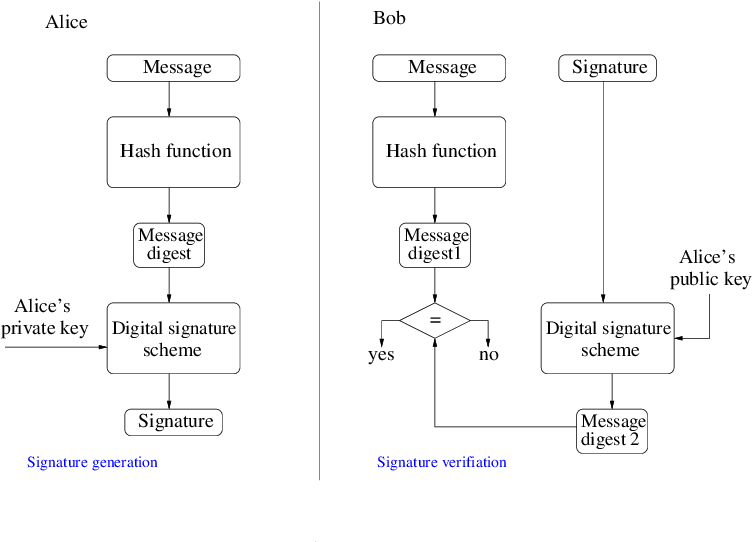
\includegraphics[width=.80\textwidth]{./Digital-signature-generation-and-verification.png}
              \caption{The General Process of Digital Signature Generation and Verification}
          \end{figure}

    \item \textbf{Which government agencies are involved to issue the digital signature? What is the validity of digital signature}\\


          \textbf{Government Agencies:}\\

          The government agencies involved in issuing digital signatures may vary depending on the country. In general, it is common for a government agency responsible for electronic signatures or digital certificates to issue digital signatures. \\

          For example, in the United States, the \textit{National Institute of Standards and Technology (NIST)} provides guidelines and standards for digital signatures and certificates.\\
    

          \textbf{Agencies in India}
          \begin{itemize}
              \item In India, digital signatures are issued by \textit{Certifying Authorities (CAs)} that are licensed by the Controller of Certifying Authorities (CCA). The CCA is a government agency under the Ministry of Electronics and Information Technology, responsible for the regulation and licensing of CAs in India. \\

              \item    The CCA is responsible for implementing the provisions of the Information Technology (IT) Act, 2000, which provides for the legal recognition of electronic records and digital signatures in India. The CCA issues licenses to CAs for issuing digital certificates, and also maintains a national repository of digital certificates that can be used to verify the authenticity of digital signatures.

              \item In addition to the CCA, the Ministry of Electronics and Information Technology and the Ministry of Law and Justice also play a role in the regulation and promotion of digital signatures and electronic transactions in India.

          \end{itemize}
          \textbf{Validity of Digital Signature:}\\

          The validity of a digital signature also varies depending on the country and the laws governing electronic signatures. In general, a digital signature is considered to be legally binding and valid if it meets certain criteria, such as:
          \begin{enumerate}

              \item The signature is created using a valid digital certificate issued by a trusted certification authority.
              \item The signer's private key is kept secure and not accessible to others.
              \item The signature was created at the time the document was signed and has not been altered since then.
              \item The certificate used to create the signature has not expired or been revoked.
              \item In most countries, digital signatures are considered to be as legally binding as traditional signatures.
              \item The validity of a digital signature can be verified by using the signer's public key to decrypt and verify the signature, and by checking the certificate used to create the signature to ensure that it is valid and has not been revoked.
          \end{enumerate}
\end{enumerate}


\chapter{Email Security using - PGP or S/MIME for Confidentiality, Authenticity and Integrity}
\section{Aim}
Demonstrate Email Security using - PGP or S/MIME for Confidentiality, Authenticity and Integrity.

\section{Objectives}
To learn authentication technique for access control

\section{Theory}

\subsection{PGP}

\begin{enumerate}
    \item PGP (Pretty Good Privacy) is a data encryption and decryption computer program that provides cryptographic privacy and authentication for data communication. PGP is used for signing, encrypting, and decrypting texts, e-mails, files, directories, and whole disk partitions and to increase the security of e-mail communications.
    \item Phil Zimmermann developed PGP in 1991. PGP and similar software follow the OpenPGP standard (RFC 4880) for encrypting and decrypting data.
    \item PGP encryption uses a serial combination of hashing, data compression, symmetric-key cryptography, and, finally, public-key cryptography; each step uses one of several supported algorithms. Each public key is bound to a user name and/or an e-mail address. The first version of this system was generally known as a web of trust to contrast with the X.509 system, which uses a hierarchical approach based on certificate authority and which was added to PGP implementations later. Current versions of PGP encryption include both options through an automated key management server.
    \item PGP encryption should only be used with data that is transferred via file transfer applications that use secure connections. PGP should not be used with email applications that send and receive data in plain text. PGP encryption is not compatible wi    
\end{enumerate}

\subsection{Steps to Send an EMail using PGP}
\subsubsection{Generate a key Pair}

The first step is to generate a key pair consisting of a private key and a public key. The private key is kept secret and is used for decrypting messages that are encrypted using the corresponding public key. The public key is shared with others so they can encrypt messages that only the owner of the private key can decrypt.

\subsubsection{Share public keys}

In order to exchange encrypted messages, each person needs to share their public key with the other person. This can be done by sharing the key through a key server, sending the key as an email attachment, or sharing it in person.
\subsubsection{Encrypt the message}

Once the public keys have been exchanged, the sender can encrypt the message using the recipient's public key. The encrypted message can only be decrypted by the recipient using their private key.
\subsubsection{Sign the message}

The sender can optionally sign the message using their private key. This adds a digital signature to the message, which provides a way for the recipient to verify that the message was actually sent by the claimed sender, and that it has not been altered in transit.
\subsubsection{Send the message}

The encrypted and optionally signed message can now be sent to the recipient through email or another messaging service.
\subsubsection{Decrypt the message}

Upon receiving the message, the recipient can decrypt it using their private key. If the message was also signed, the recipient can verify the digital signature using the sender's public key.

These steps are shown below in Input and outputs.

\section{Platform}
\textbf{\textbf{Operating System}}: Arch Linux x86-64 \\
\textbf{\textbf{IDEs or Text Editors Used}}: Visual Studio Code\\

\section{Input and Output}

\subsection{Generated Keys}

\lstinputlisting[language=bash, caption="Krish Private Key"]{../Programs/Assignment_8/krish_private_key.txt}

\lstinputlisting[language=bash, caption="Krish Public Key"]{../Programs/Assignment_8/krish_public_key.txt}

\begin{figure}[H]
    \centering
    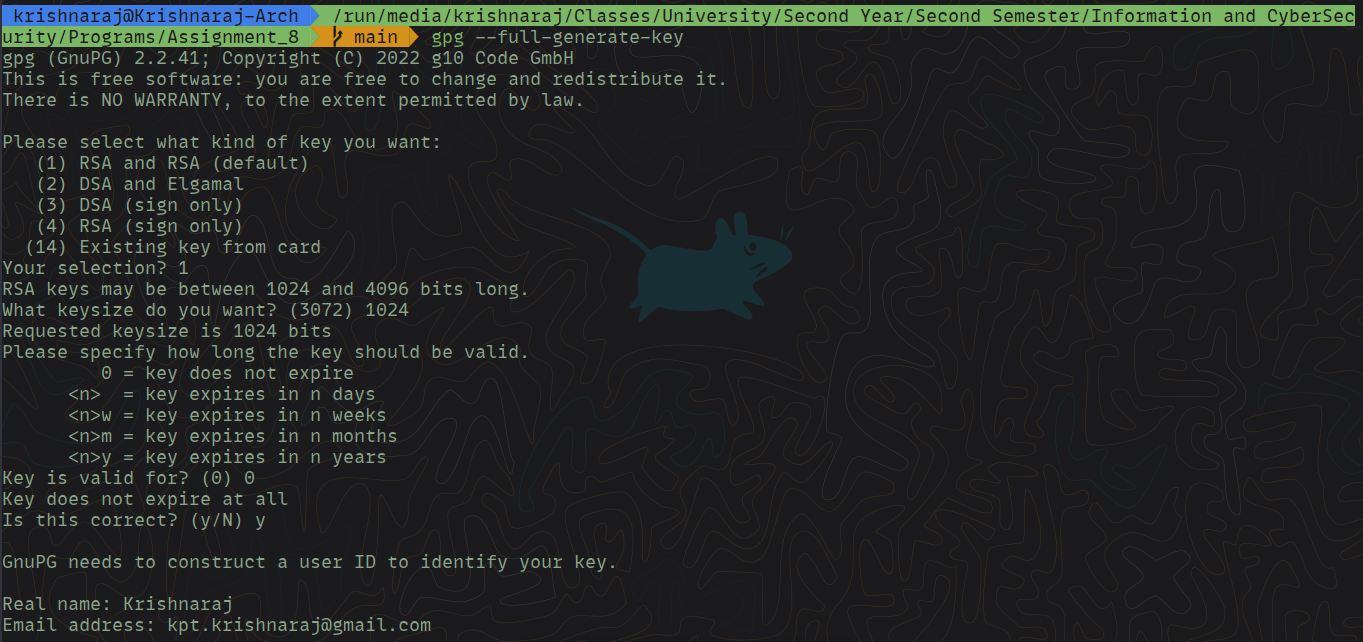
\includegraphics[width=1\textwidth]{../Programs/Assignment_8/Screenshot_on_2023-04-13_at_12-28-59.png}
    \caption{Generating Key Pairs}
\end{figure}
\begin{figure}[H]
    \centering
    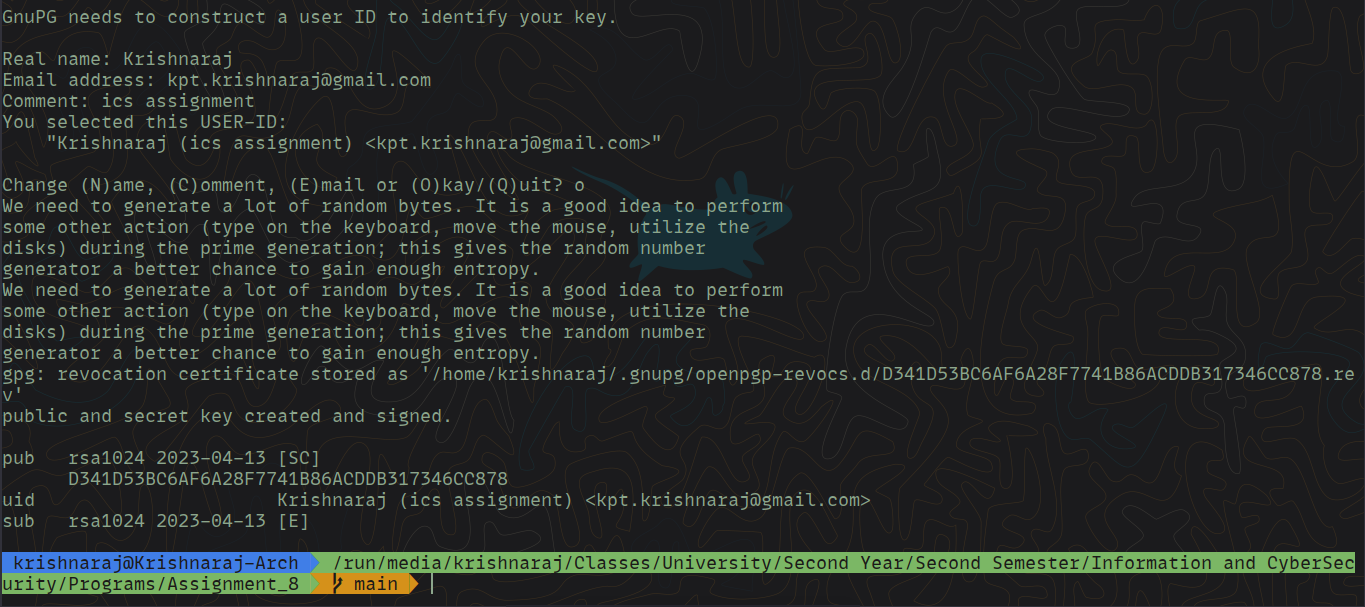
\includegraphics[width=.99\textwidth]{../Programs/Assignment_8/Screenshot_on_2023-04-13_at_12-29-06.png}
    \caption{Generating Key Pairs continued}
\end{figure}
\begin{figure}[H]
    \centering
    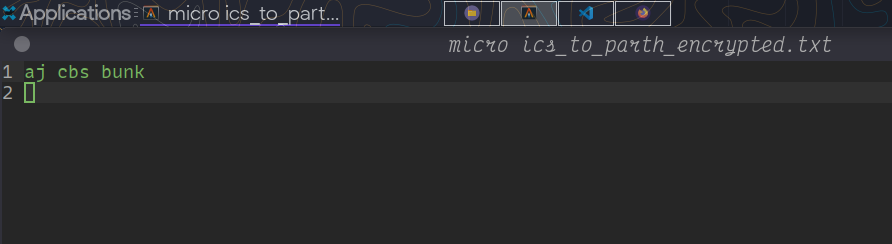
\includegraphics[width=.99\textwidth]{../Programs/Assignment_8/Screenshot_on_2023-04-13_at_12-29-34.png}
    \caption{Secret Message to Parth - Recipient - "Aj CBS Bunk"}
\end{figure}
\begin{figure}[H]
    \centering
    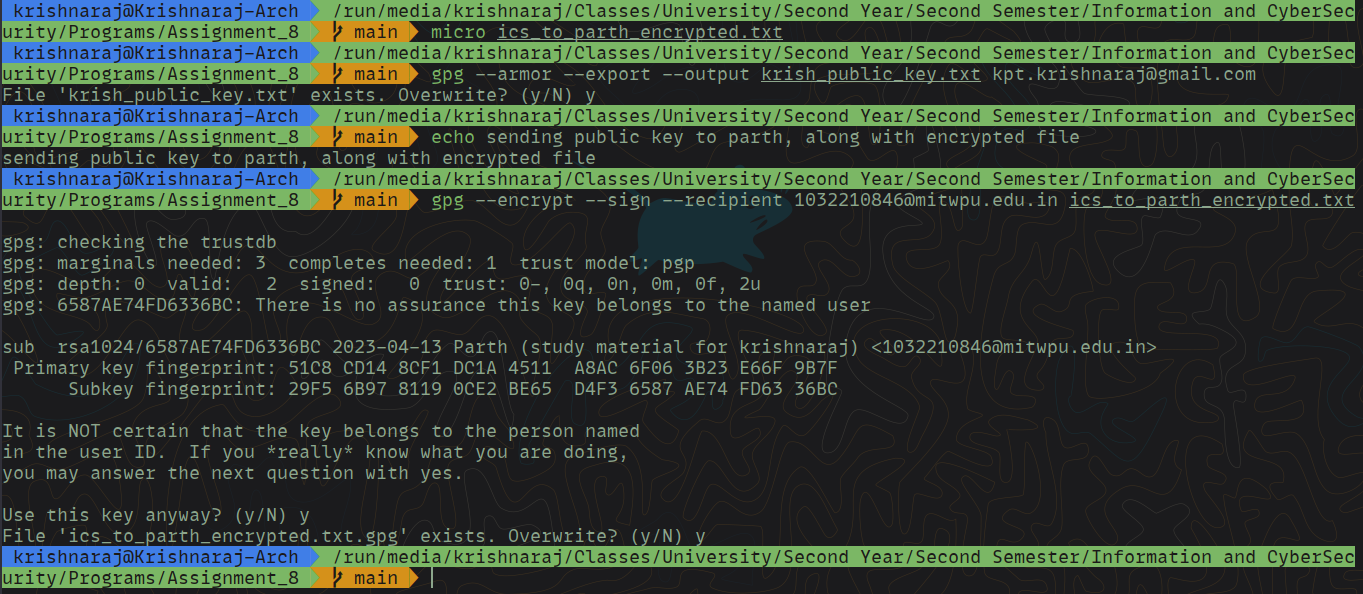
\includegraphics[width=.99\textwidth]{../Programs/Assignment_8/Screenshot_on_2023-04-13_at_12-31-43.png}
    \caption{Signing Message to Send Parth using Parth's Public Key}
\end{figure}
\begin{figure}[H]
    \centering
    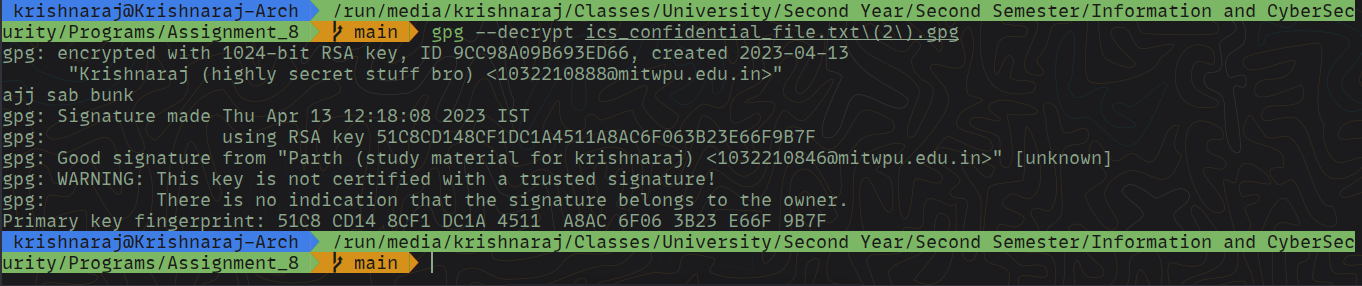
\includegraphics[width=.99\textwidth]{../Programs/Assignment_8/Screenshot_on_2023-04-13_at_12-32-03.png}
    \caption{Decrypting Message from Parth using his Public key - "Ajj Sab Bunk"}
\end{figure}

\begin{verbatim}

\end{verbatim}


% \section{Code}
% \lstinputlisting[language=Python, caption="DSA Signature Validity using PyCrypto Library"]{../Programs/Assignment_7/dsa using lib.py}

\section{Conclusion}
Thus, we have successfully implemented Email Security using - PGP or S/MIME for Confidentiality, Authenticity and Integrity.
\clearpage

\section{FAQ}

\begin{enumerate}
    \item \textbf{How email security is provided through PGP?}\\

          \begin{enumerate}
              \item PGP (Pretty Good Privacy) provides email security through a combination of encryption, digital signatures, and compression. When a user sends an email using PGP, the message is encrypted using a symmetric key algorithm.

              \item The symmetric key is then encrypted using the recipient's public key, which is obtained from a key server or a public key directory. The encrypted message and the encrypted symmetric key are then sent to the recipient, who can decrypt the message using their private key.

              \item PGP also allows users to sign their emails digitally using their private key. The digital signature provides a way for the recipient to verify that the email was actually sent by the claimed sender, and that it has not been altered in transit.
              \item In addition, PGP can compress the message before encryption, which can reduce the size of the message and make it easier to send over a slow or unreliable connection.
          \end{enumerate}

    \item \textbf{What type of encryption is PGP?}\\

          PGP uses a combination of symmetric and asymmetric encryption. The symmetric encryption algorithm is used to encrypt the message itself, while the asymmetric encryption algorithm is used to encrypt the symmetric key.\\

          The symmetric encryption algorithm used in PGP is typically AES (Advanced Encryption Standard), which is a widely used and highly secure algorithm. The asymmetric encryption algorithm used in PGP is typically RSA (Rivest–Shamir–Adleman), which is also widely used and highly secure.

    \item \textbf{What is the key size allowed in PGP}\\

          PGP supports a wide range of key sizes, from 512 bits to 4096 bits. The key size determines the level of security provided by the encryption algorithm.\\

          In general, larger key sizes provide stronger security, but they also require more processing power to encrypt and decrypt the data. For most purposes, a key size of 2048 bits is considered to be sufficient, but some applications may require larger key sizes for enhanced security.


\end{enumerate}



\chapter{Secured web applications system using SSL certificates and its deployment in Apache Tomcat Server}
\section{Aim}

Demonstration of secured web applications system using SSL certificates and its
deployment in Apache tomcat server

\section{Objectives}
To learn different vulnerability scanning.

\section{Theory}

\subsection{SSL Certificate}
An SSL (Secure Sockets Layer) certificate is a digital certificate that verifies the authenticity of a website and encrypts data transmitted between the website and the user's web browser. SSL certificates ensure that all sensitive information, such as usernames, passwords, and credit card numbers, are transmitted securely over the internet.

\subsection{How does an SSL certificate work?}
When a user visits a website that has an SSL certificate, the website's server sends the user's web browser a copy of the certificate. The browser then verifies the certificate with the Certificate Authority (CA) that issued it. If the certificate is valid, the browser establishes a secure connection with the website using SSL/TLS encryption.

\subsection{Types of SSL certificates}
There are different types of SSL certificates based on the number of domains or subdomains they cover, the level of validation, and the warranty offered by the Certificate Authority (CA). Some common types of SSL certificates include:

\begin{enumerate}
    \item Domain Validated (DV) SSL Certificate: This type of SSL certificate only validates the domain name of the website, ensuring that it belongs to the entity requesting the certificate. DV SSL certificates are the most common type of SSL certificate and are suitable for personal websites or blogs.
    \item Organization Validated (OV) SSL Certificate: This type of SSL certificate validates both the domain name and the identity of the organization or business requesting the certificate. OV SSL certificates are suitable for e-commerce websites and other online businesses.
    \item Extended Validation (EV) SSL Certificate: This type of SSL certificate provides the highest level of validation and requires extensive documentation to prove the identity of the organization requesting the certificate. EV SSL certificates are suitable for large businesses and financial institutions.
    \item Wildcard SSL Certificate: This type of SSL certificate covers multiple subdomains of a single domain name. For example, a wildcard SSL certificate for the domain example.com would cover subdomains such as blog.example.com and shop.example.com.
\end{enumerate}

\subsection{Benefits of SSL certificates}

There are several benefits of using an SSL certificate for a website, including:
\begin{enumerate}
    \item Data encryption: SSL certificates encrypt all data transmitted between the website and the user's web browser, ensuring that sensitive information is secure.
    \item Authentication: SSL certificates provide authentication, verifying that the website is legitimate and belongs to the entity requesting the certificate.
    \item Trust and credibility: SSL certificates display trust indicators, such as the padlock icon in the web browser's address bar, which can increase a website's credibility and reputation.
    \item SEO benefits: SSL certificates can improve a website's search engine ranking, as search engines prefer secure websites.
    \item

\end{enumerate}
\subsection{Example}
Suppose you want to create an e-commerce website where users can purchase products and enter their personal information, such as name, address, and credit card details. To ensure that the website is secure and trustworthy, you decide to obtain an SSL certificate.\\

You choose to purchase an OV SSL certificate, which will validate your domain name and your business's identity. You submit your company's legal documents and undergo a validation process to prove your identity.\\

Once the CA verifies your documents and identity, they issue the SSL certificate, which you install on your website's server. Now, when users visit your website, their web browsers will establish a secure connection using SSL/TLS encryption, ensuring that their personal information is protected.

\section{Platform}
\textbf{\textbf{Operating System}}: Arch Linux x86-64 \\
\textbf{\textbf{IDEs or Text Editors Used}}: Visual Studio Code\\

\section{Input and Output}
\begin{figure}[H]
    \centering
    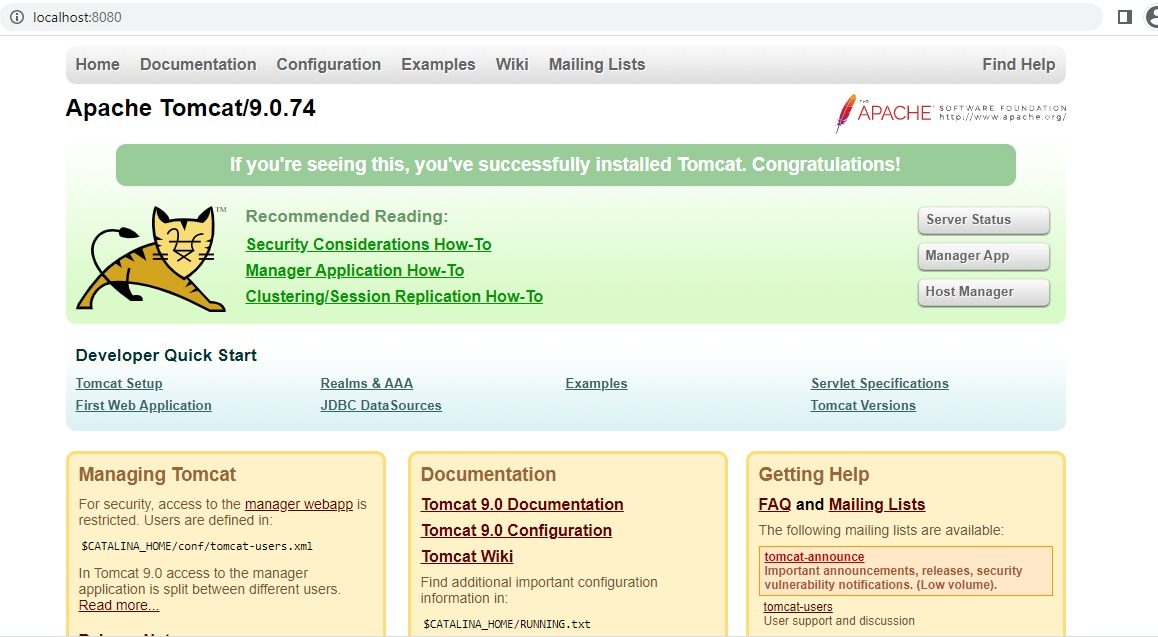
\includegraphics[width=.95\textwidth]{tomcat.jpeg}
    \caption{}
\end{figure}
\begin{figure}[H]
    \centering
    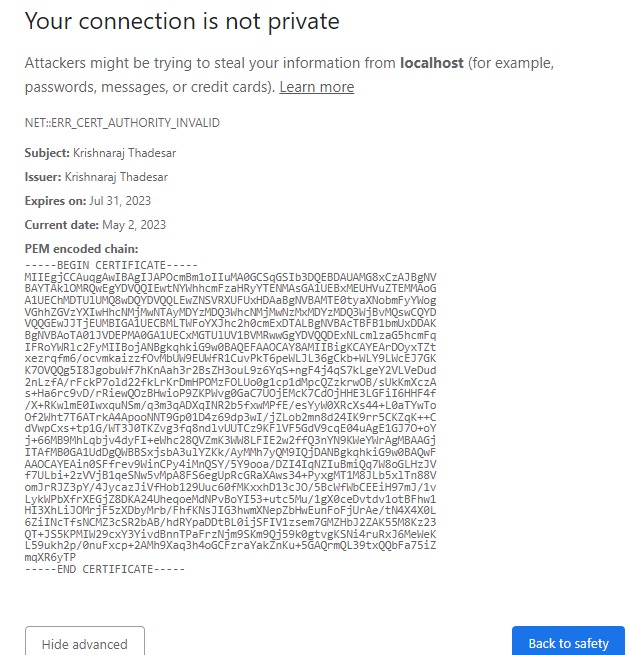
\includegraphics[width=.95\textwidth]{tomcat1.jpeg}
    \caption{}
\end{figure}
\begin{figure}[H]
    \centering
    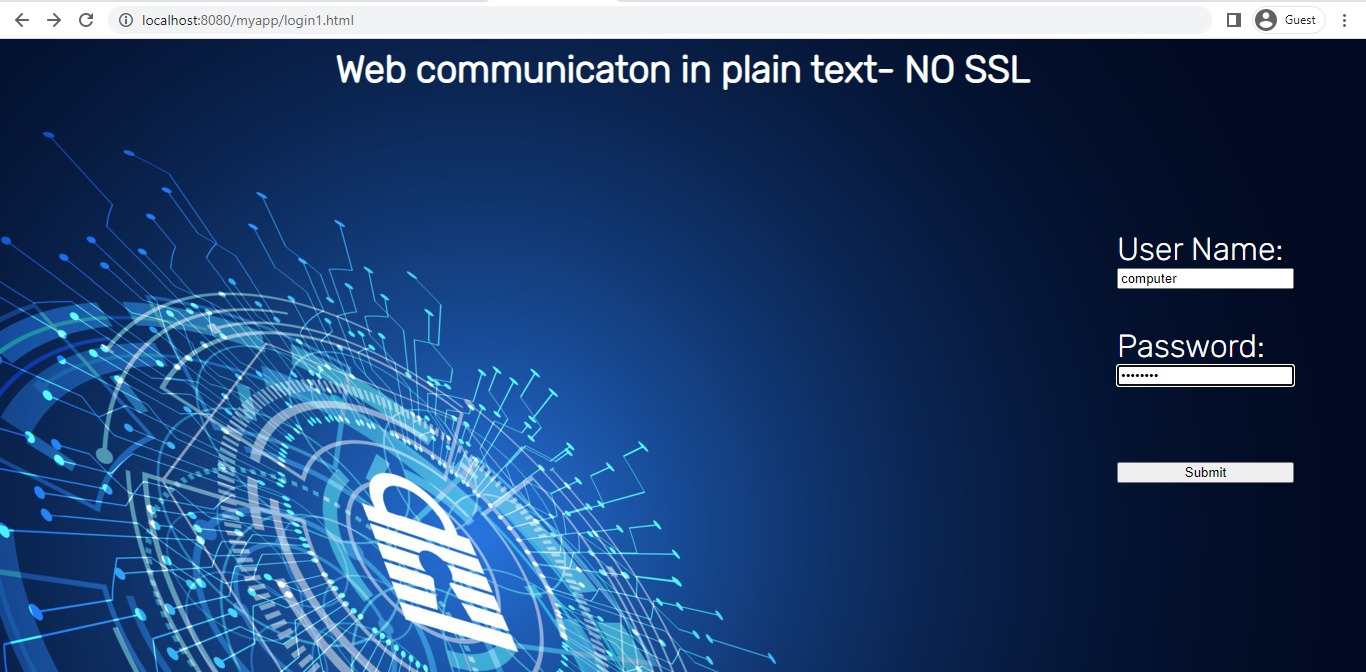
\includegraphics[width=.95\textwidth]{tomcat2.jpeg}
    \caption{}
\end{figure}
\begin{figure}[H]
    \centering
    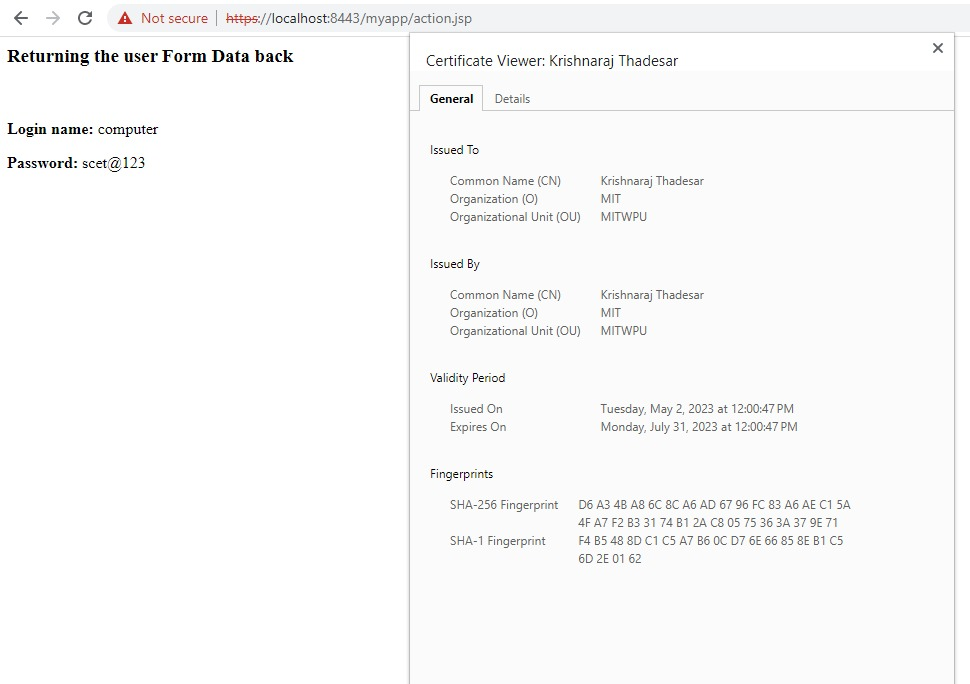
\includegraphics[width=.95\textwidth]{tomcat3.jpeg}
    \caption{}
\end{figure}
\begin{verbatim}
The Given Signature is Valid
\end{verbatim}


% \section{Code}
% \lstinputlisting[language=Python, caption="DSA Signature Validity using PyCrypto Library"]{../Programs/Assignment_7/dsa using lib.py}

\section{Conclusion}
Thus, we have successfully implemented
\clearpage

\section{FAQ}

\begin{enumerate}
    \item \textbf{What type of encryption does SSL use?}\\

          Secure Socket Layer (SSL) uses a combination of symmetric and asymmetric encryption to secure data transmitted over a network. SSL uses asymmetric encryption during the initial handshake process, where the client and server exchange public keys to establish a secure communication channel. Once the secure channel is established, SSL uses symmetric encryption to encrypt the data being transmitted between the client and server.\\

          Symmetric encryption uses a single secret key to encrypt and decrypt data, while asymmetric encryption uses a pair of keys, one private and one public. The public key can be freely shared, while the private key is kept secret. In SSL, the public key is used to encrypt the data, and the private key is used to decrypt the data.\\

          SSL supports a variety of symmetric encryption algorithms, including AES, DES, and 3DES. It also supports a variety of asymmetric encryption algorithms, including RSA, DSA, and ECDSA.

    \item \textbf{How safe is SSL?}\\

          SSL is generally considered to be a secure protocol for transmitting sensitive data over a network. SSL has undergone multiple revisions over the years, with the latest version being Transport Layer Security (TLS). TLS version 1.3 is the latest and most secure version of SSL/TLS, which has been designed to provide strong encryption and better security features.\\

          However, SSL can be vulnerable to various types of attacks, such as Man-in-the-Middle (MITM) attacks, where an attacker intercepts the communication between the client and server and eavesdrops on the conversation or alters the data being transmitted. SSL is also vulnerable to attacks that exploit weaknesses in the encryption algorithms or the SSL protocol itself.\\

          To mitigate these risks, SSL implementations must be properly configured and maintained to ensure they are up-to-date with the latest security patches and best practices. It is also recommended to use SSL/TLS certificates from trusted Certificate Authorities (CA) and to use strong passwords and multi-factor authentication to protect the private keys used for encryption.

    \item \textbf{What are the benefits of SSL?}\\

          The benefits of SSL include:

          \begin{enumerate}
              \item Data encryption: SSL encrypts the data transmitted between the client and server, which helps to protect the data from unauthorized access and eavesdropping.
              \item Authentication: SSL uses digital certificates to authenticate the identity of the server and ensure that the client is communicating with the intended server.
              \item Trust: SSL/TLS certificates are issued by trusted Certificate Authorities (CA) that verify the identity of the server and ensure that the SSL/TLS certificate is valid.
              \item Compliance: SSL is required by many industry regulations and compliance standards, such as the Payment Card Industry Data Security Standard (PCI DSS).
              \item Improved search engine ranking: Google has confirmed that HTTPS is a ranking factor, and using SSL/TLS can help to improve search engine rankings.
          \end{enumerate}

\end{enumerate}



\chapter{Intrusion Detection System using Snort}
\section{Aim}
Configuration and demonstration of Intrusion Detection System using Snort

\section{Objectives}
To learn authentication techniques for Access Control


\section{Theory}

Host-based IDS (HIDS) and Network-based IDS (NIDS) are two types of intrusion detection systems that are used to monitor and detect potential security threats.

\subsection{HIDS - Host-based IDS}

A Host-based IDS (HIDS) is an IDS system that is installed on individual hosts or endpoints to monitor the activity on that host. It uses system logs, file integrity checks, and other methods to identify potential security threats. The HIDS can detect attacks that are not visible on the network, such as local privilege escalation, malware infections, and unauthorized access attempts.\\

Example: OSSEC is an open-source HIDS that can detect various host-based attacks, including rootkits, file changes, and unauthorized access attempts. It uses a combination of signature-based, anomaly-based, and heuristic-based detection methods to increase the accuracy of attack detection and reduce false positives.

\subsection{NIDS - Network-based IDS}

A Network-based IDS (NIDS) is an IDS system that is installed on the network to monitor traffic passing through it. It analyzes packets passing through the network to identify suspicious behavior, such as unusual traffic patterns, unauthorized access attempts, and malware infections. NIDS can detect attacks that are visible on the network, but may not detect attacks that are targeted to a specific host or endpoint.\\

Example: Snort is an open-source NIDS that can detect a wide range of attacks and anomalies in network traffic. It uses a combination of signature-based, anomaly-based, and heuristic-based detection methods to increase the accuracy of attack detection and reduce false positives. Suricata is another open-source NIDS that can detect various network-based attacks, including DDoS, malware infections, and suspicious traffic patterns.\\

HIDS and NIDS can be used together to provide a comprehensive security solution. While HIDS is good at detecting attacks on a specific host or endpoint, NIDS can detect attacks that are not visible on the host or endpoint. Using both HIDS and NIDS can help provide a layered security approach to detect and respond to potential security threats.


\begin{figure}[H]
    \centering
    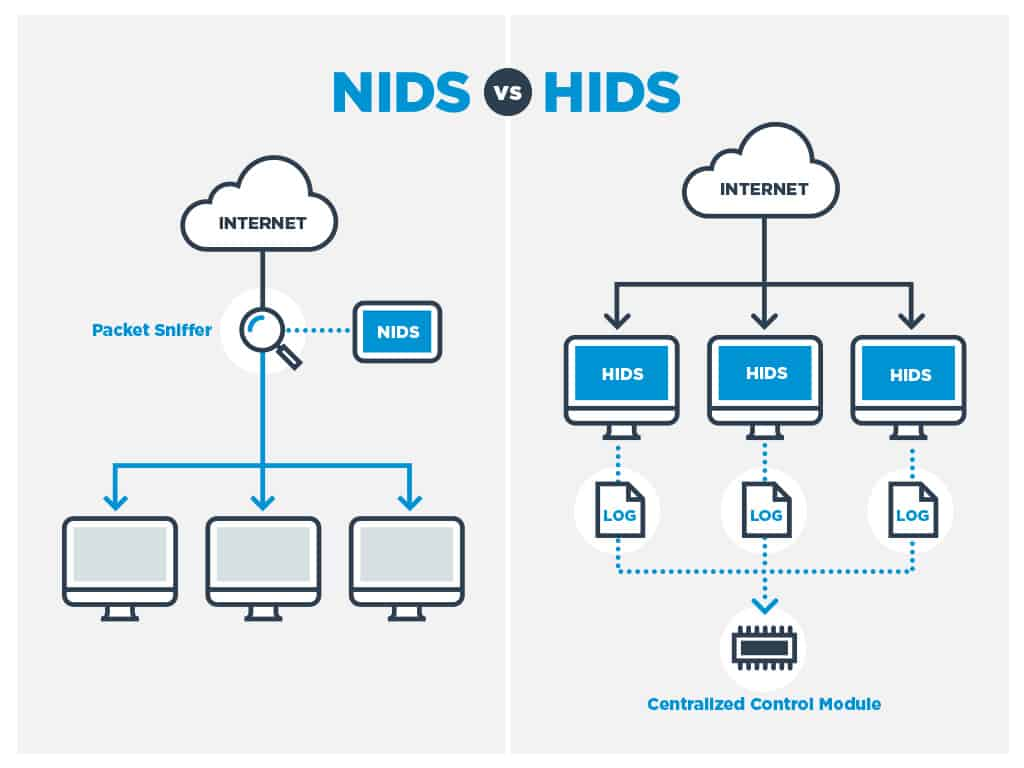
\includegraphics[width=.85\textwidth]{NIDS-vs-HIDS.jpg}
\end{figure}
\section{Platform}
\textbf{Operating System}: Arch Linux x86-64 \\
\textbf{IDEs or Text Editors Used}: Visual Studio Code\\
\textbf{Compilers or Interpreters}: Python 3.10.1\\

\section{Input and Output}
\begin{figure}[H]
    \centering
    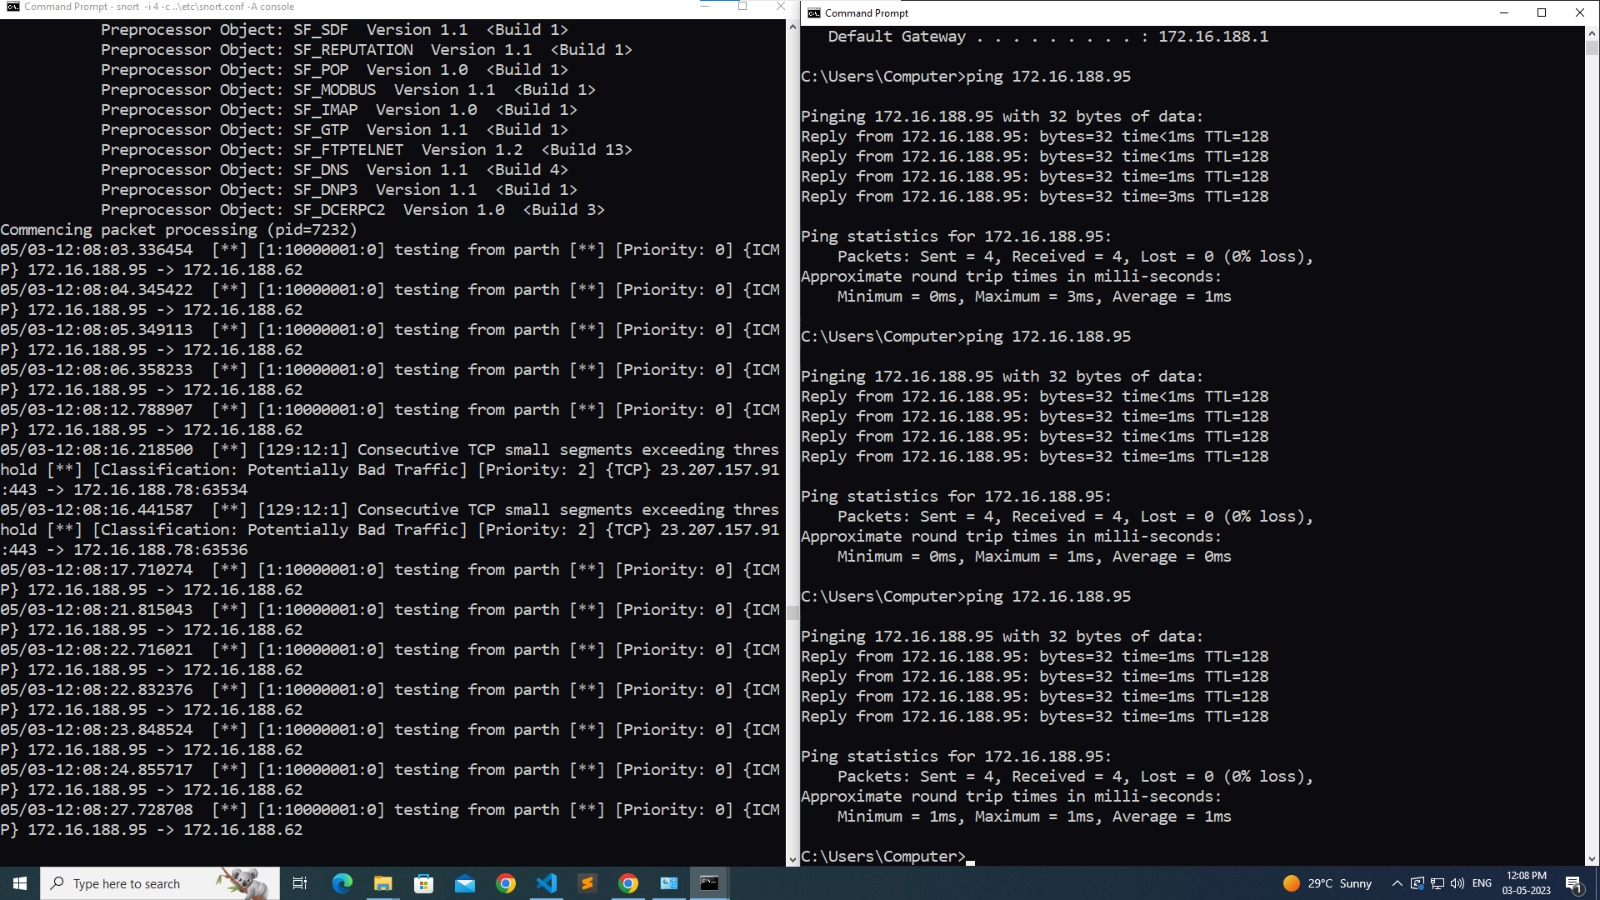
\includegraphics[width=.95\textwidth]{snort1.jpeg}
    \caption{}
\end{figure}
\begin{figure}[H]
    \centering
    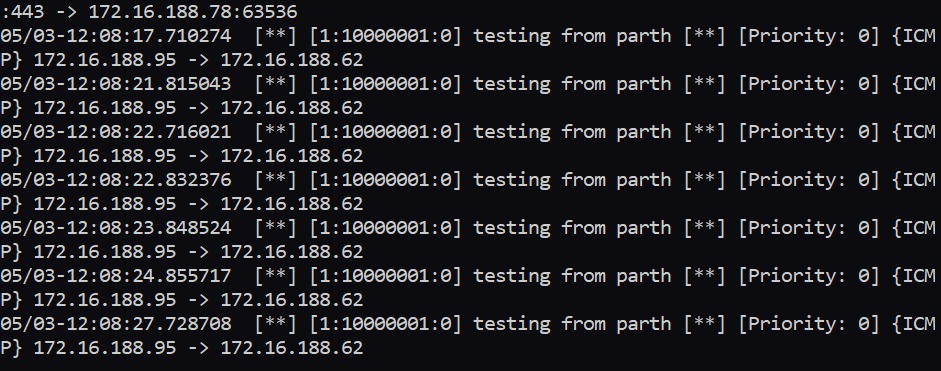
\includegraphics[width=.95\textwidth]{snort2.jpeg}
    \caption{}
\end{figure}
\begin{figure}[H]
    \centering
    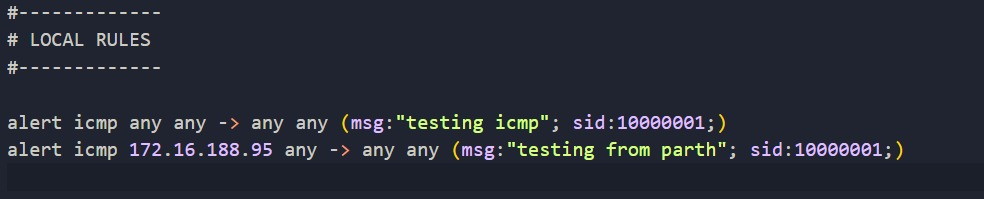
\includegraphics[width=.95\textwidth]{snort3.jpeg}
    \caption{}
\end{figure}
\begin{verbatim}
% The Given Signature is Valid
\end{verbatim}

% \section{Code}
% \lstinputlisting[language=Python, caption="DSA Signature Validity using PyCrypto Library"]{../Programs/Assignment_7/dsa using lib.py}

\section{Conclusion}
Thus, We have learnt IDS systems and their types. We have also learnt about various tools based on IDS systems.
\clearpage

\section{FAQ}

\begin{enumerate}
    \item \textbf{What are various types of IDS system?}\\

          There \textit{are two main types of IDS systems}:
          \begin{enumerate}
              \item \textit{Network-based IDS (NIDS)}: NIDS systems monitor network traffic in real-time to detect and alert on potential attacks. They analyze packets passing through the network to identify suspicious behavior, such as unusual traffic patterns, unauthorized access attempts, and malware infections.
              \item \textit{Host-based IDS (HIDS)}: HIDS systems monitor the activity on individual hosts to detect and alert on potential attacks. They analyze system logs, file integrity, and user activity to identify suspicious behavior, such as unauthorized access, malware infections, and changes to system configurations.
          \end{enumerate}

    \item \textbf{What are the popular tools based on IDS systems?}\\

          There \textit{are several popular tools based on IDS systems, including}:

          \begin{enumerate}
              \item \textit{Snort}: an open-source NIDS that can detect a wide range of attacks and anomalies in network traffic.
              \item \textit{Suricata}: an open-source NIDS that can detect and alert on various network-based attacks, including DDoS, malware infections, and suspicious traffic patterns.
              \item \textit{OSSEC}: an open-source HIDS that can detect and alert on various host-based attacks, including rootkits, file changes, and unauthorized access attempts.
              \item \textit{Bro}: an open-source NIDS that can detect and alert on various network-based attacks, including malware infections, network scans, and suspicious traffic patterns.
              \item \textit{Security Onion}: a Linux distribution that includes several IDS tools, including Snort, Suricata, and Bro, and provides a centralized platform for monitoring and analyzing network and host activity.
          \end{enumerate}

    \item \textbf{What are the detection methods of IDS?}\\
          IDS systems use several methods for detecting potential attacks, including:
          \begin{enumerate}
              \item \textit{Signature-based detection}: IDS systems can detect known attacks by comparing network or host activity to a database of known attack signatures. If a match is found, the IDS can generate an alert.
              \item \textit{Anomaly-based detection}: IDS systems can detect new or unknown attacks by identifying patterns or behavior that deviate from normal or expected activity. This method requires a baseline of normal activity to be established, which the IDS can then use to identify anomalies.
              \item \textit{Heuristic-based detection}: IDS systems can detect potential attacks by using algorithms and rules to identify behavior that is indicative of an attack. This method can be more flexible than signature-based detection, but can also result in more false positives.
              \item \textit{Hybrid detection}: IDS systems can use a combination of signature-based, anomaly-based, and heuristic-based detection methods to increase the accuracy of attack detection and reduce false positives.
          \end{enumerate}


\end{enumerate}



\chapter{NESSUS tool for Vulnerability Assessment}
\section{Aim}
Configuration and demonstration of NESSUS tool for vulnerability assessment

\section{Objectives}
To learn authentication technique for access control

\section{Theory}
\subsection{Vulnerability Assessment}
Vulnerability assessment is the process of identifying and evaluating potential security vulnerabilities in a computer system or network. This assessment helps organizations to identify and prioritize potential risks and develop strategies to mitigate them. One of the popular vulnerability assessment tools is Nessus.\\

Nessus is a widely used vulnerability assessment tool that is designed to scan and detect vulnerabilities in networks, systems, and applications. Here are some of the features of Nessus:
\begin{enumerate}
    \item Multiple scanning options: Nessus offers various scanning options, including network, web application, and database scanning. It supports multiple protocols, such as TCP/IP, SNMP, SSH, and HTTP/HTTPS.
    \item Comprehensive vulnerability database: Nessus maintains a comprehensive database of known vulnerabilities and exploits, which it uses to identify potential vulnerabilities in the target system.
    \item Customizable policies: Nessus allows users to customize scan policies based on their specific needs. Users can create policies to scan specific IP addresses, ports, or protocols.
    \item Real-time alerts: Nessus provides real-time alerts on critical vulnerabilities, enabling organizations to quickly remediate potential threats.
    \item Compliance reporting: Nessus generates compliance reports based on industry standards such as PCI DSS, HIPAA, and CIS.
    \item Integration with other tools: Nessus can integrate with other security tools such as SIEMs and incident response platforms.

\end{enumerate}

\subsection{How Nessus Works}
\begin{enumerate}
    \item Discovery: Nessus starts by discovering devices on the network, including servers, workstations, routers, and switches.
    \item Scan configuration: The user configures the scan policy based on their needs, such as IP range, scanning ports, protocols, and vulnerabilities to scan for.
    \item Scan execution: Nessus then scans the target system for vulnerabilities based on the configured policy. The scanning process may take some time, depending on the size of the network and the complexity of the scan policy.
    \item Vulnerability assessment: Nessus then analyzes the scan results and reports potential vulnerabilities. It provides detailed information on the type of vulnerability, the level of severity, and possible remediation actions.
    \item Reporting: Nessus generates a report that summarizes the vulnerabilities found during the scan. The report includes detailed information on each vulnerability, including its severity level and recommended remediation actions.
\end{enumerate}

\section{Platform}
\textbf{\textbf{Operating System}}: Arch Linux x86-64 \\
\textbf{\textbf{IDEs or Text Editors Used}}: Visual Studio Code\\
\textbf{\textbf{Compilers or Interpreters} }: Python 3.10.1\\

\section{Input and Output}
\begin{figure}[H]
    \centering
    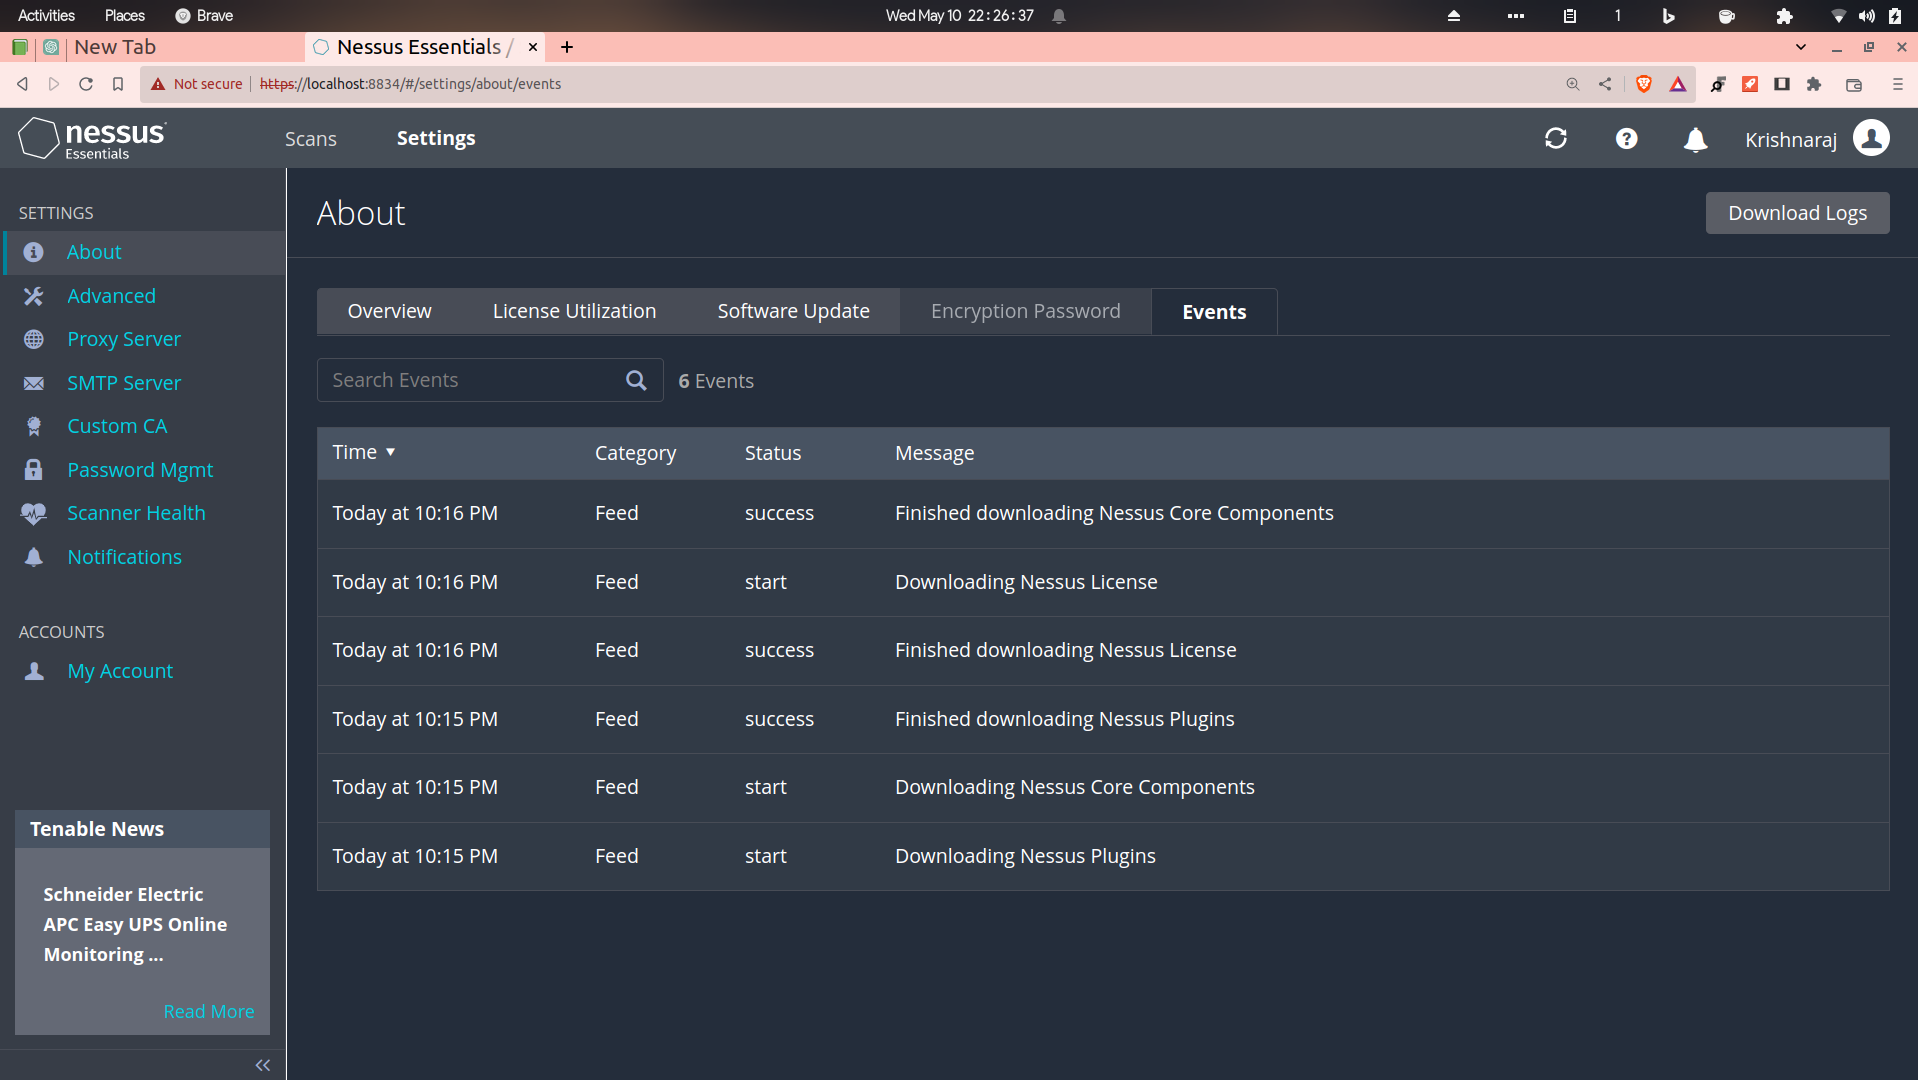
\includegraphics[width=.95\textwidth]{nessus 1.png}
    \caption{Nessus Home Page}
\end{figure}
\begin{figure}[H]
    \centering
    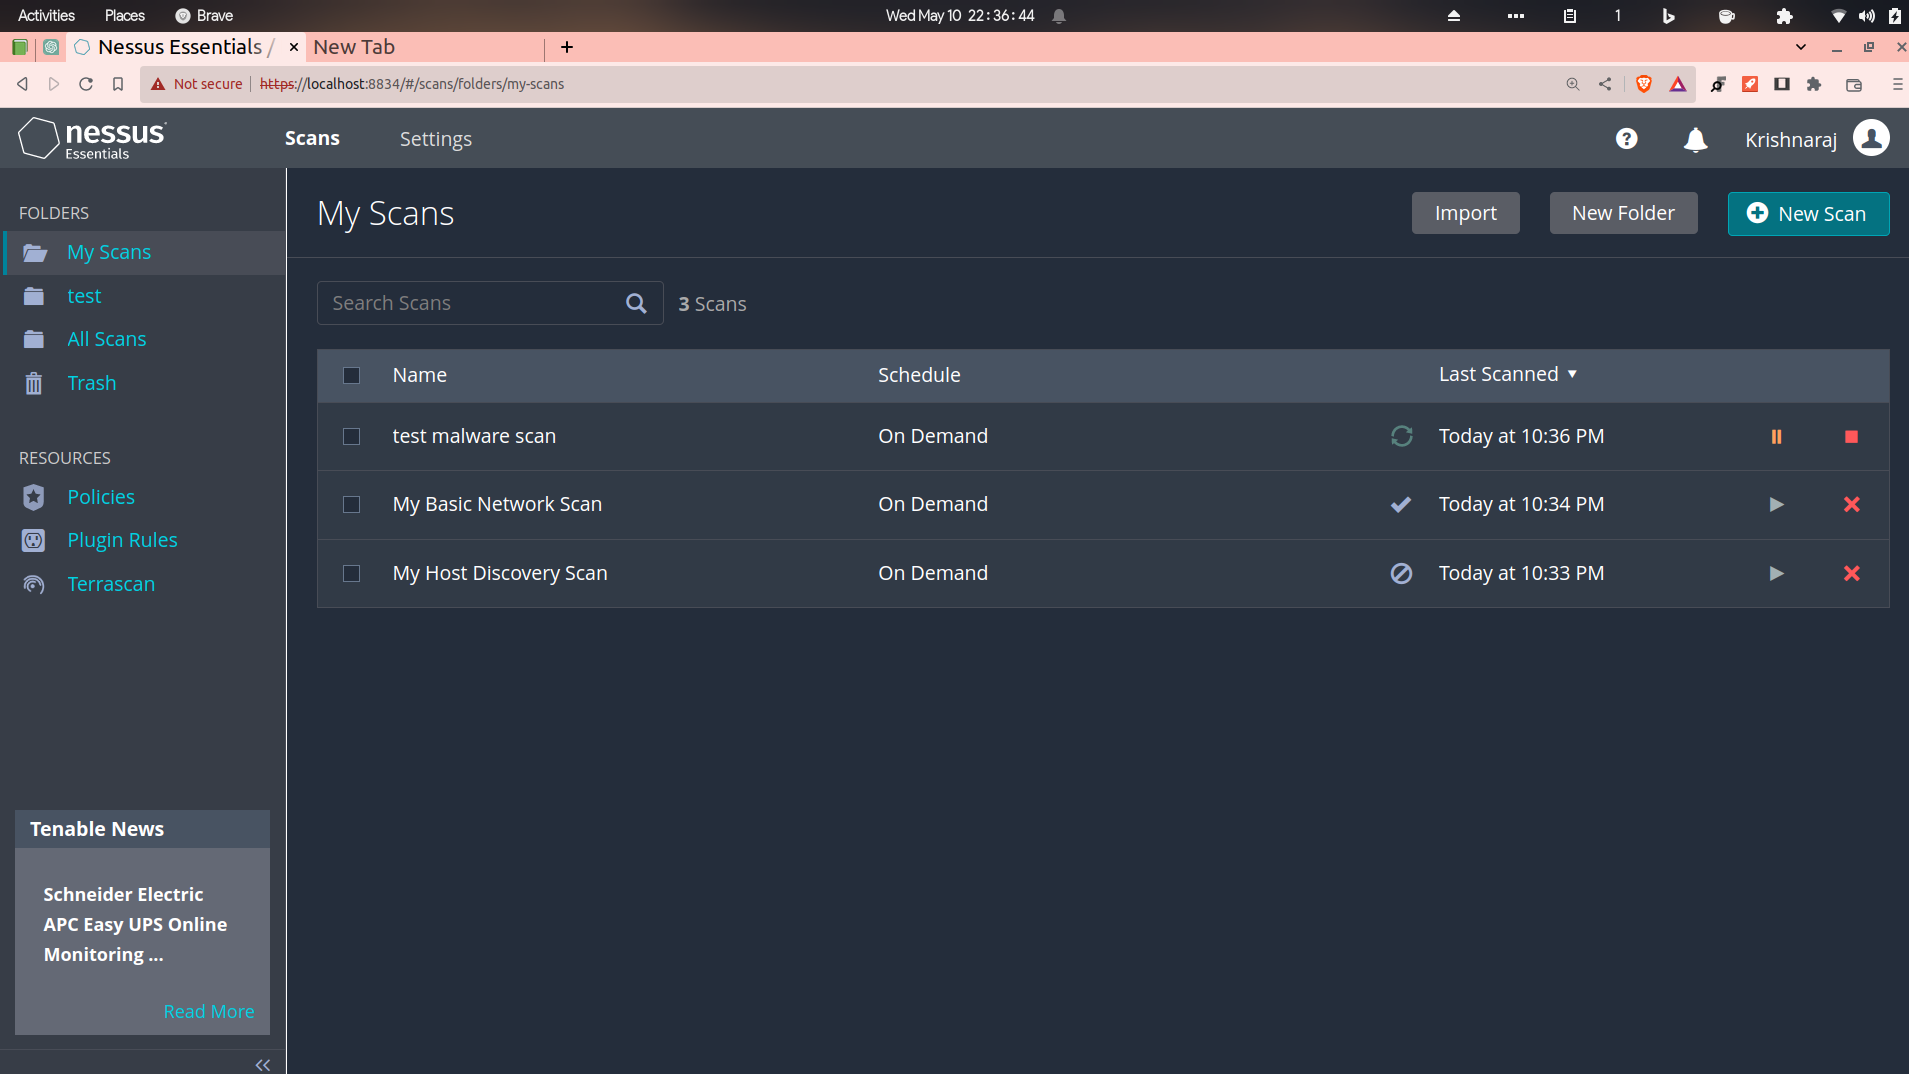
\includegraphics[width=.95\textwidth]{nessus 2.png}
    \caption{Nessus Scans}
\end{figure}
\begin{verbatim}
\end{verbatim}


% \section{Code}
% \lstinputlisting[language=Python, caption="DSA Signature Validity using PyCrypto Library"]{../Programs/Assignment_7/dsa using lib.py}

\section{Conclusion}
Thus, we have learnt about the authentication technique for access control, and implemented it using NESSUS tool for vulnerability assessment.Thus, we have seen how to implement digital signatures using DSA algorithm.
\clearpage

\section{FAQ}

\begin{enumerate}

    \item \textbf{What vulnerabilities can Nessus detect?}\\

          Nessus is a vulnerability scanner that can detect a wide range of vulnerabilities in an IT environment, including:

          \begin{enumerate}
              \item Operating system vulnerabilities: Nessus can identify vulnerabilities in the operating systems of network devices, servers, and workstations, including Windows, Linux, Unix, and macOS.
              \item Application vulnerabilities: Nessus can detect vulnerabilities in popular applications such as web browsers, email clients, and office productivity software.
              \item Network vulnerabilities: Nessus can identify network vulnerabilities, including weak passwords, open ports, and misconfigured network devices.
              \item Malware and botnets: Nessus can detect signs of malware and botnets on network devices and workstations.
              \item Web application vulnerabilities: Nessus can identify vulnerabilities in web applications, including SQL injection, cross-site scripting, and directory traversal.
          \end{enumerate}
    \item \textbf{What are the limitations of Nessus essentials?}\\

          Nessus Essentials is a free version of the Nessus vulnerability scanner that is limited in its capabilities compared to the paid version. Some of the limitations of Nessus Essentials include:

          \begin{itemize}
              \item Limited scanning: Nessus Essentials is limited to scanning up to 16 IP addresses or hosts at a time, while the paid version can scan thousands of hosts.
              \item No scheduling: Nessus Essentials does not allow users to schedule scans or automated reporting, which can be inconvenient for organizations with large IT environments.
              \item Limited vulnerability coverage: Nessus Essentials has a smaller set of plugins for detecting vulnerabilities compared to the paid version, which can limit its effectiveness in identifying security issues.
              \item No support: Nessus Essentials does not come with technical support from Tenable, the company behind Nessus.
          \end{itemize}
    \item \textbf{How can you identify a false positive vulnerability in Nessus?}\\

          A false positive vulnerability in Nessus occurs when the scanner reports a vulnerability that does not actually exist. To identify false positive vulnerabilities in Nessus, follow these steps:

          \begin{itemize}
              \item Verify the vulnerability: Check the affected device or application to verify if the reported vulnerability actually exists.
              \item Check the plugin output: Review the Nessus plugin output to identify any discrepancies or errors that may have led to the false positive.
              \item Confirm with multiple sources: Check other vulnerability scanners, security advisories, and technical forums to confirm if the vulnerability is a known issue.
              \item Perform additional testing: Conduct additional testing or penetration testing to confirm if the vulnerability can be exploited.
          \end{itemize}

    \item \textbf{How many hosts can Nessus scan? What port does Nessus use?}\\

          The number of hosts that Nessus can scan depends on the version of the software and the license purchased. The free version of Nessus, Nessus Essentials, can scan up to 16 IP addresses or hosts at a time, while the paid versions can scan thousands of hosts.\\

          Nessus uses various ports to communicate with the devices being scanned. The default port used by Nessus is 8834 for web-based communication, but Nessus can also use other ports depending on the type of scan being performed. For example, Nessus may use port 22 for SSH communication or port 445 for SMB communication.
\end{enumerate}

\end{document}
